\documentclass[12pt]{article}
\usepackage[T2A]{fontenc}
\usepackage[utf8]{inputenc}
\usepackage{multirow}
\usepackage{caption}
\usepackage{subcaption}
\usepackage{amsmath}
\usepackage{changepage}
\usepackage{graphicx}
\usepackage{float}
\usepackage[english,russian]{babel}
\usepackage{amsmath, amsfonts, amssymb, amsthm, mathtools}
\usepackage{xcolor}
\usepackage{array}
\usepackage{hyperref}
\usepackage[top = 1.5cm, left = 1.5 cm, right = 1.5 cm, bottom = 3 cm]{geometry}
\graphicspath{ {./images/} }
 
\title{Измерение вязкости воздуха по течению в тонких трубах}
\author{Шахматов Андрей, Б02-304}
\date{\today}
  
\begin{document}
\begin{titlepage}
    \begin{center}
        {\large МОСКОВСКИЙ ФИЗИКО-ТЕХНИЧЕСКИЙ ИНСТИТУТ (НАЦИОНАЛЬНЫЙ ИССЛЕДОВАТЕЛЬСКИЙ УНИВЕРСИТЕТ)}
    \end{center}
    \begin{center}
        {\large Физтех-школа физики и исследований им. Ландау}
    \end{center}
    
    
    \vspace{3cm}
    {\huge
        \begin{center}
            \textbf{Измерение вязкости воздуха по течению в тонких трубах}
        \end{center}
    }
    \vspace{2cm}
    \begin{flushright}
        {\LARGE Автор:\\ Шахматов Андрей Юрьевич \\
            \vspace{0.2cm}
            Б02-304}
    \end{flushright}
    \vspace{7 cm}
    \begin{center}
        Долгопрудный 2024
    \end{center}
\end{titlepage}

% \maketitle

\begin{abstract}
    Исследована зависимость потока воздуха $Q$ через тонкие трубки в зависимости от перепада давления 
    на концах трубки $P$. По полученным данным определён коэффициент вязкости воздуха при нормальных условиях. 
    Измерено распределение давления в трубке при ламинарном течении воздуха.      
\end{abstract}

\tableofcontents

\section{Введение}
Цель настоящей работы заключалась в определении коэффициента вязкости воздуха при нормальных условиях.

\section{Методика}
\subsection*{Теоретическая справка}
Рассмотрим движение вязкой жидкости или газа по трубке круглого сечения. При малых скоростях потока движение оказывается ламинарным (слоистым), скорости частиц меняются по радиусу и направлены вдоль оси трубки. С увеличением скорости потока движение становится турбулентным, и слои перемешиваются. При турбулентном движении скорость в каждой точке быстро меняет величину и направление, сохраняется только средняя величина скорости.

Характер движения газа (или жидкости) в трубке определяется безразмерным числом Рейнольдса:
\[Re = \dfrac{\upsilon r \rho}{\eta} \text{  } \text{  } \text{  }(1)\]
где $\upsilon$ - скорость потока, $r$ - радиус трубки, $\rho$ - плотность движущейся среды, $\eta$ - вязкость. В гладких трубах круглого сечения переход от ламинарного движения к турбулентному происходит при $Re \approx 1000$

При ламинарном течении объем газа $V$, протекающий за время $t$ по трубе длиной $l$, определяется формулой Пуазейля:
\[Q_V = \dfrac{\pi r^4}{8 l \eta}(P_1 - P_2) \text{  } \text{  } \text{  }(2)\]
В этой формуле $P_1 - P_2$ - разность давлений в двух выбранных сечениях 1 и 2, расстояние между которыми равно $l$. Велечину $Q$ обычно называют расходом. Формула (2) позволяет определять вязкость газа по его расходу.

Отметим условия, при которых справедлива формула (2). Прежде всего необходимо, чтобы с достаточным запасом выполнялось неравенство $Re < 1000$. Необходимо также, чтобы при течении не происходило существенного изменения удельного объема газа (при выводе формулы удельный объем считался постоянным). Для жидкости это предположение выполняется практически всегда, а для газа - лишь в тех случаях, когда перепад давлений вдоль трубки мал по сравнению с самим давлением. В нашем случае давление газа равно атмосферному ($10^3$ см вод. ст.), а перепад давлений составляет не более 10 см вод. ст., то есть менее $1\%$ от атмосферного. Формула (2) выводится для участков трубки, на которых закон распределения скоростей газа по сечению не меняется при движении вдоль потока.
\begin{figure}[H]
  \begin{center}
    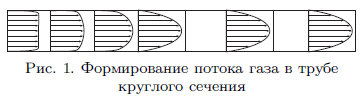
\includegraphics[width = 0.6\textwidth]{133_1.png}
  \end{center}
\end{figure}
При втекании газа в трубку из большого резервуара скорости слоев вначале постоянны по всему сечению (рис. 1). По мере продвижения газа по трубке картина распределения скоростей меняется, так как сила трения о стенку тормозит прилежащие к ней слои. Характерное для ламинарного течения параболическое распределение скоростей устанавливается на некотором расстоянии $a$ от входа в трубку, которое зависит от радиуса трубки $r$ и числа Рейнольдса по формуле
\[a \approx  0,2 r \cdot Re \text{ } \text{ } \text{ } (3)\]
Градиент давления на участке формирования потока оказывается большим, чем на участке с установившимся ламинарным течением, что позволяет разделить эти участки экспериментально. Формула (3) дает возможность оценить длину участка формирования.
\subsection*{Экспериментальная установка}
\begin{figure}[H]
    \begin{center}
      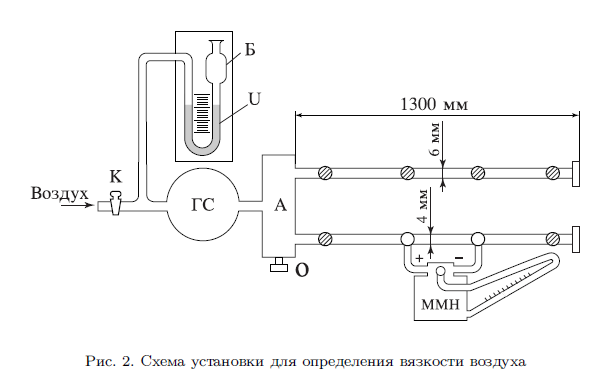
\includegraphics[width = 0.6\textwidth]{133_2.png}
    \end{center}
\end{figure}
Измерения производятся на экспериментальной установке, схема которой изображена на рис. 2. Поток воздуха под давлением, несколько превышающим атмосферное (на 5-7 см вод. ст.), через газовый счетчик ГС поступает в резервуар А, к которому припаяны тонкие металлические трубки. Примерные размеры трубок указаны на рисунке (точные размеры обозначены на установке). Обе трубки на концах снабжены заглушками, не пропускающими воздух. Во время измерений заглушка открывается только на рабочей трубке; конец другой трубки должен быть плотно закрыт. Перед входом в газосчётчик поставлена U-образная трубка, наполовину заполненная водой. Она выполняет две задачи. Первая - измерение давления газа на входе в газосчётчик. Вторая - предохранение газосчётчика от выхода из строя. Дело в том, что газосчётчик устойчиво работает, если давление газа на его входе не превышает 600 мм водяного столба. Высота U-образной трубки примерно 600 мм, поэтому, когда давление на входе в счётчик превышает 600 мм водяного столба,вода из U-образной трубки выплёскивается в защитный баллон Б и, создавая шум, привлекает к себе внимание экспериментатора.

\section{Результаты и их обсуждение}
\subsection*{Определение коэффициента вязкости воздуха}
В эксперименте опыт проводился на трёх тонких трубках различных диаметров (Прил. \ref{app_1}). Для каждой 
из трубок измерена зависимость потока воздуха $Q$, протекающего через трубку от перепада давления $P$ (Таблица \ref{tab:1}).
Для трубки диаметром $3.95$ мм построен график зависимости $Q(P)$(Рис. \ref{fig:PQd1}).  
\begin{figure}[H]
    \centering
    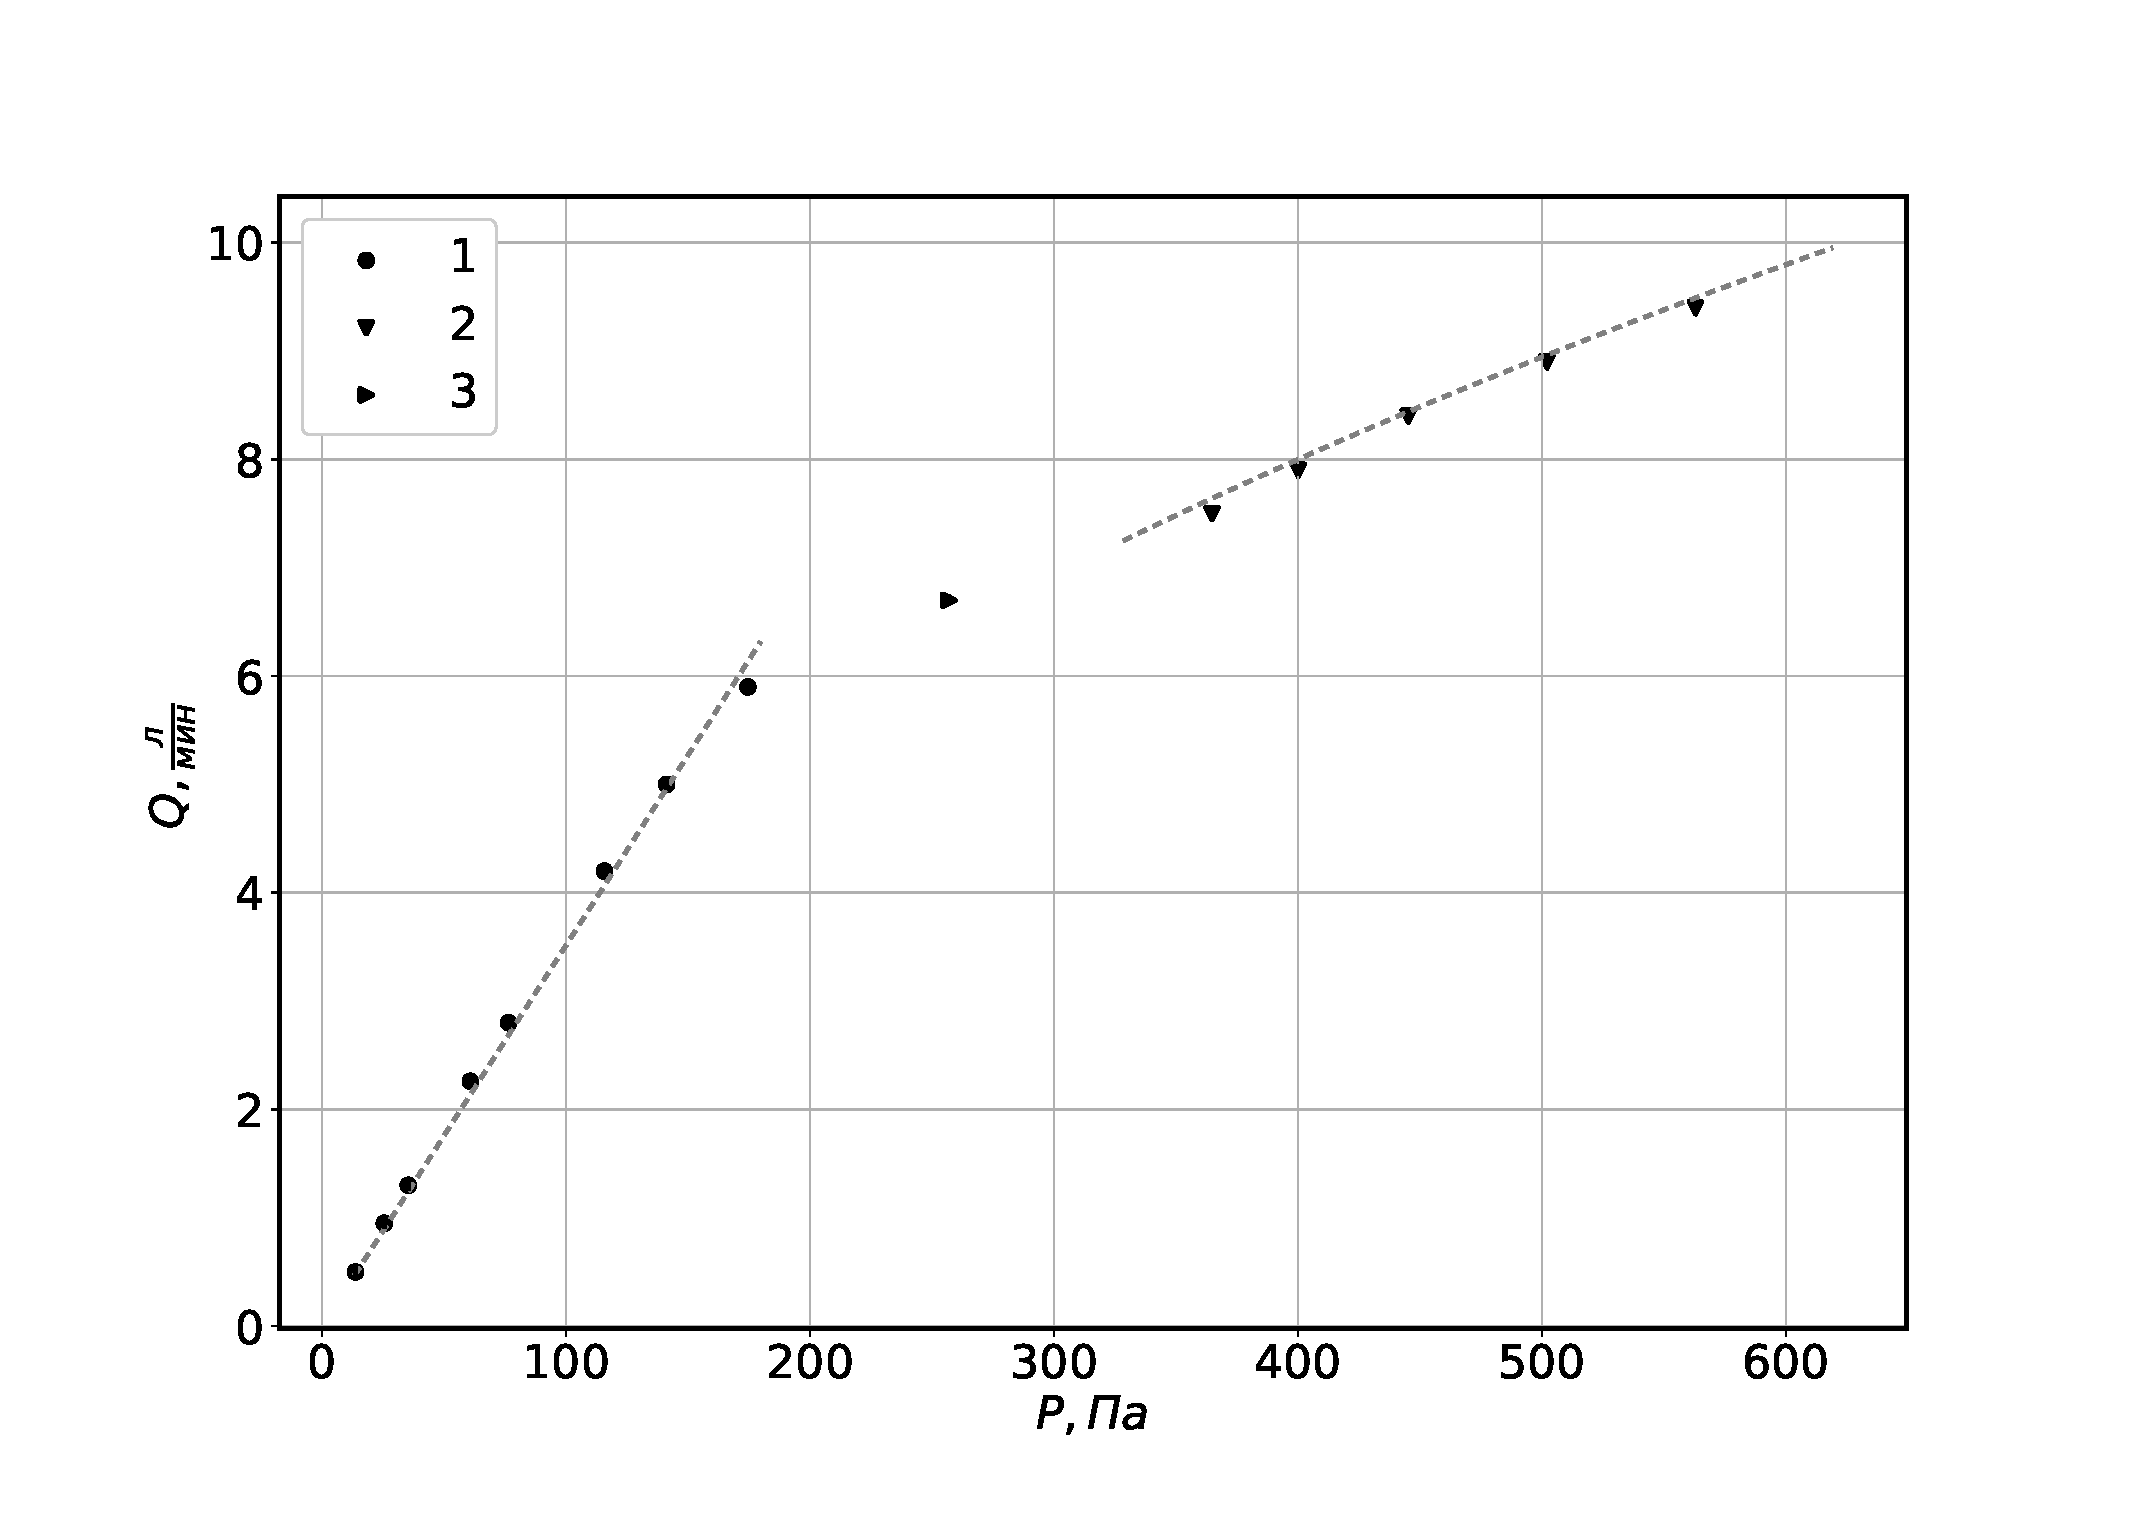
\includegraphics[width=0.8\textwidth]{PQd1.eps}
    \caption{Зависимость потока воздуха через трубку $Q$ в зависимости от перепада давления на концах
        трубки $P$. Диаметр трубки $d_1 = 3.95$ мм. Длина трубки $l_1 = 50$ см. Цифрами на графике обозначены 
        участки газа, удовлетворяющие различным режимам течения газа: 
        1 - ламинарное течение газа,
        2 - турбулентный переходное течение газа, 
        3 - турбулентное установившиеся течение газа.}
    \label{fig:PQd1}
\end{figure}
На графике видно три участка, удовлетворяющие различным режимаам течения газа в трубе. Для дальнейшего 
анализа построен график в логарифмическом масштабе (Рис. \ref{fig:lnPlnQd1}). На нём можно выделить три участка:
линейный с коэффициентом наклона равным $1$ - ламинарное течение газа, нелинейный переходной участок, 
отвечающий турбулентному неустойчивому режиму и линейный участок с коэффициентом наклона равным $\frac{1}{2}$ - 
устойчивое турбулентное течение газа. Существование таких режимов и характер их зависимостей совпадает с 
предложенной теоретической моделью.  
\begin{figure}[H]
    \centering
    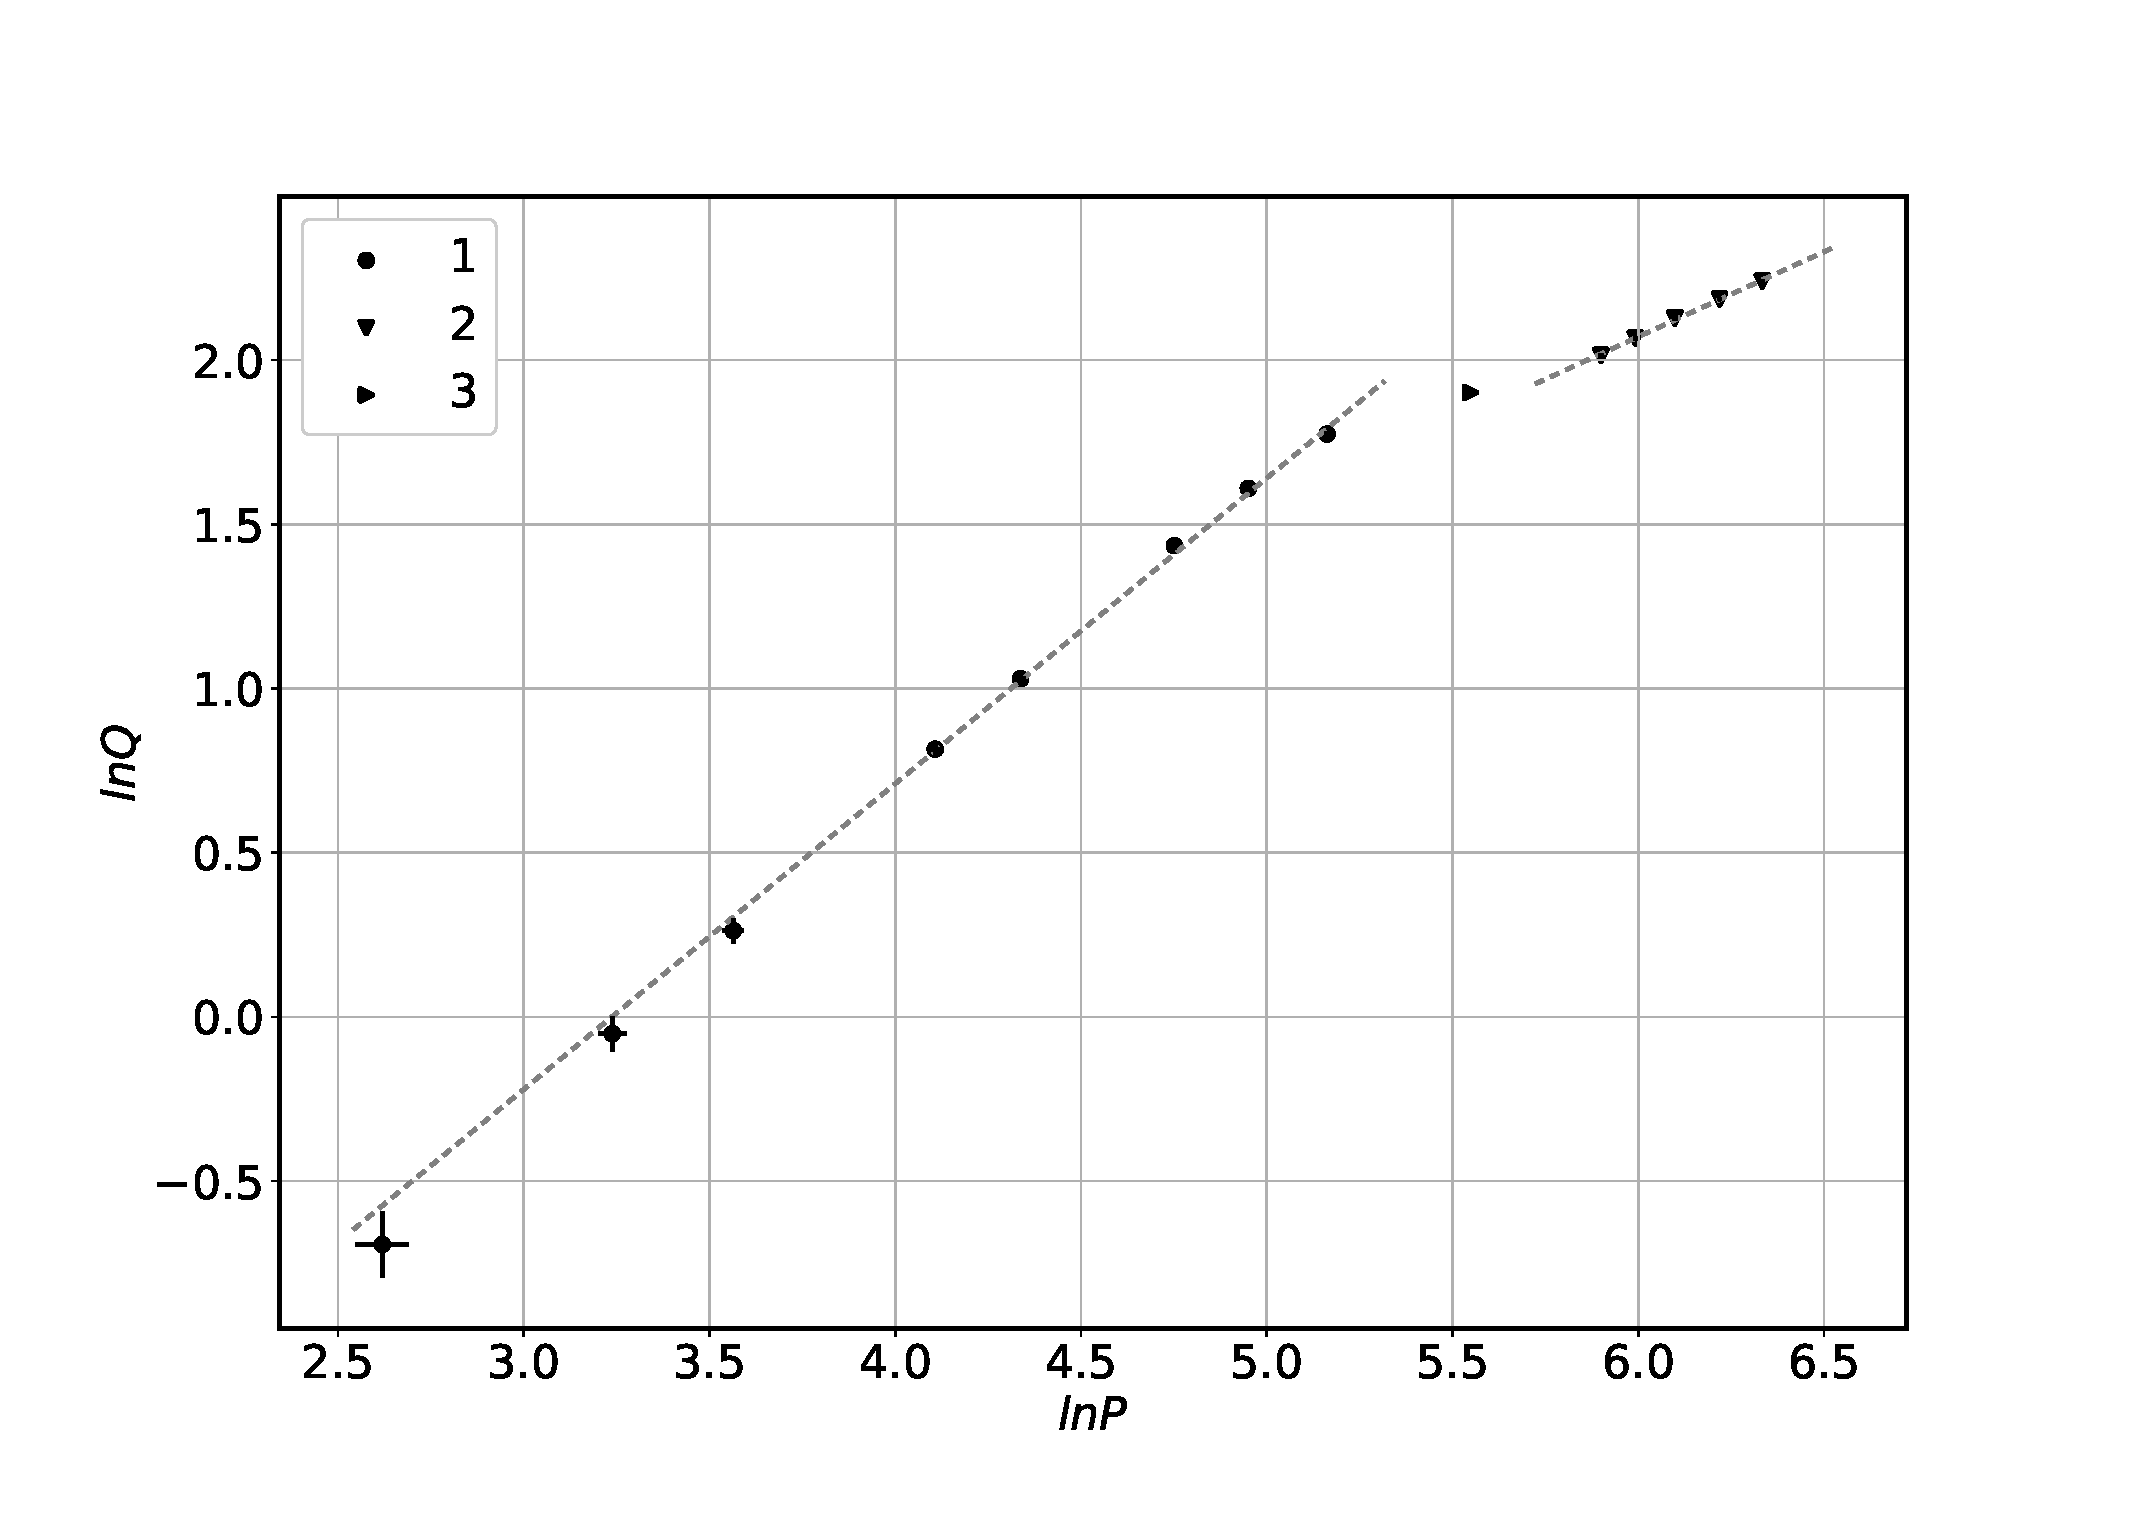
\includegraphics[width=0.8\textwidth]{lnPlnQd1.eps}
    \caption{Зависимость потока воздуха через трубку $Q$ в зависимости от перепада давления на концах
        трубки $P$ в логарифмическом масштабе. Диаметр трубки $d_1 = 3.95$ мм. Длина трубки $l_1 = 50$ см. Цифрами на графике обозначены 
        участки газа, удовлетворяющие различным режимам течения газа: 
        1 - ламинарное течение газа,
        2 - турбулентный переходное течение газа,
        3 - турбулентное установившиеся течение газа.}
    \label{fig:lnPlnQd1}
\end{figure}
Для трубки диаметром $3$ мм построен график зависимости $Q(P)$ (Рис. \ref{fig:PQd2}), 
а также график в логарифмическом масштабе (Рис. \ref{fig:lnPlnQd2}). Для данной трубки 
отсутствует явно выраженный переходной режим, который присутствовал для трубки диаметром $3.95$ мм.  
\begin{figure}[H]
    \centering
    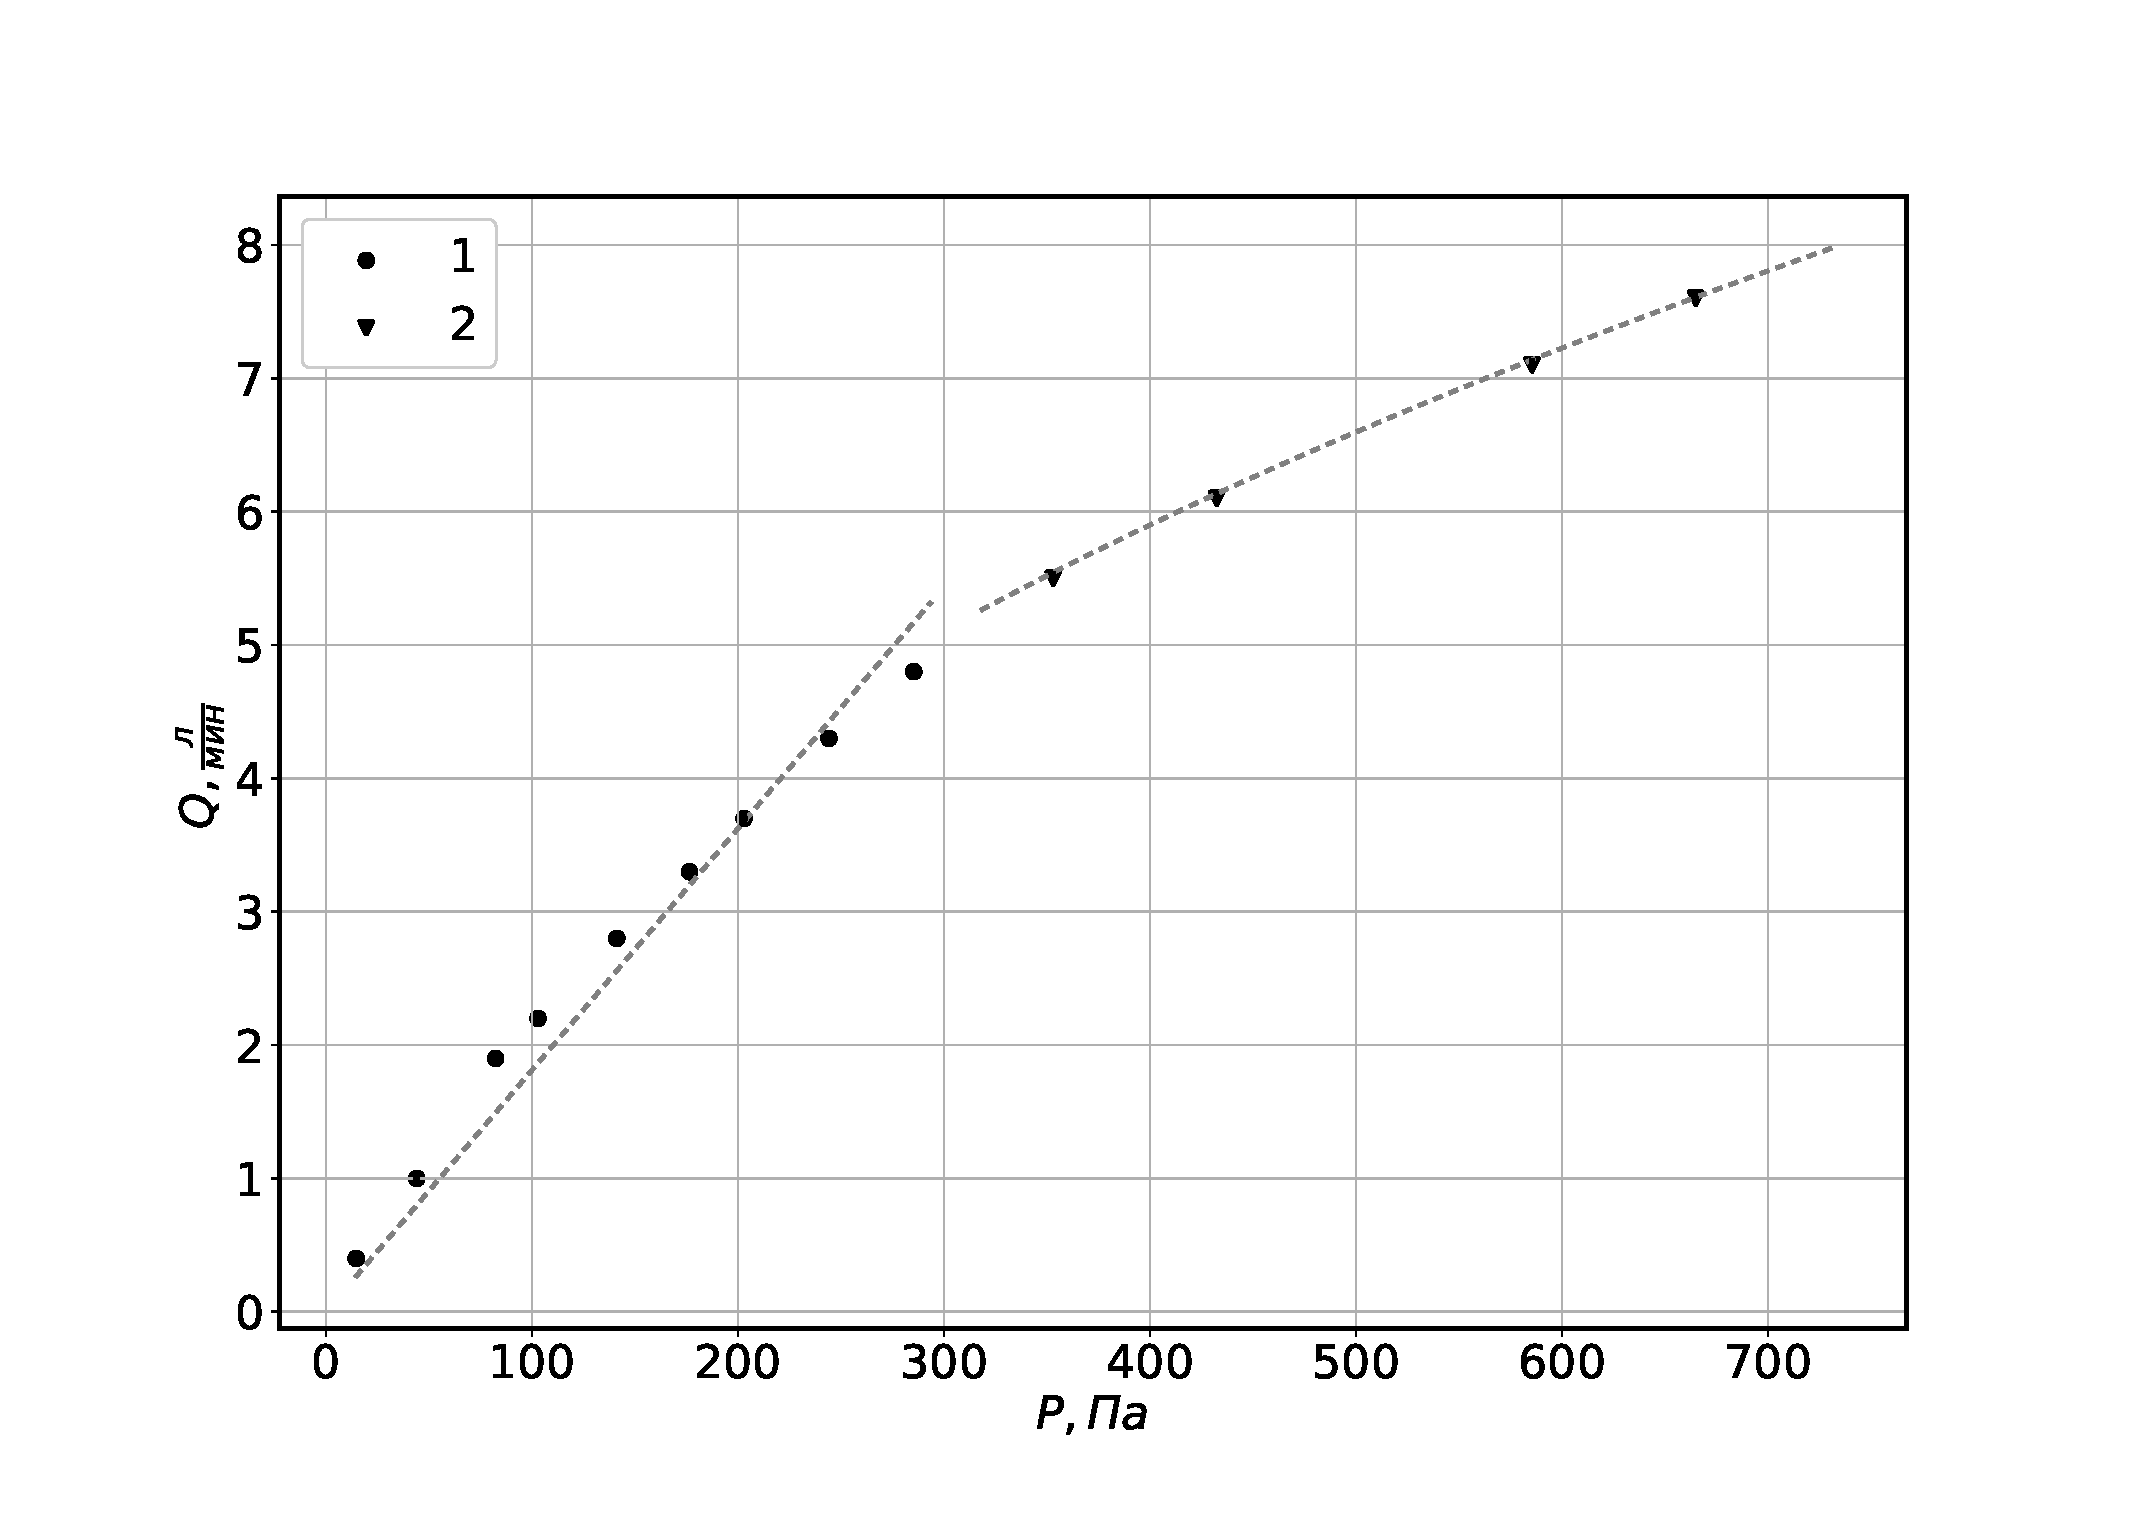
\includegraphics[width=0.8\textwidth]{PQd2.eps}
    \caption{Зависимость потока воздуха через трубку $Q$ в зависимости от перепада давления на концах
        трубки $P$. Диаметр трубки $d_2 = 3$ мм. Длина трубки $l_2 = 30$ см. Цифрами на графике обозначены 
        участки газа, удовлетворяющие различным режимам течения газа: 
        1 - ламинарное течение газа,
        2 - турбулентный переходное течение газа, 
        3 - турбулентное установившиеся течение газа.}
    \label{fig:PQd2}
\end{figure}
\begin{figure}[H]
    \centering
    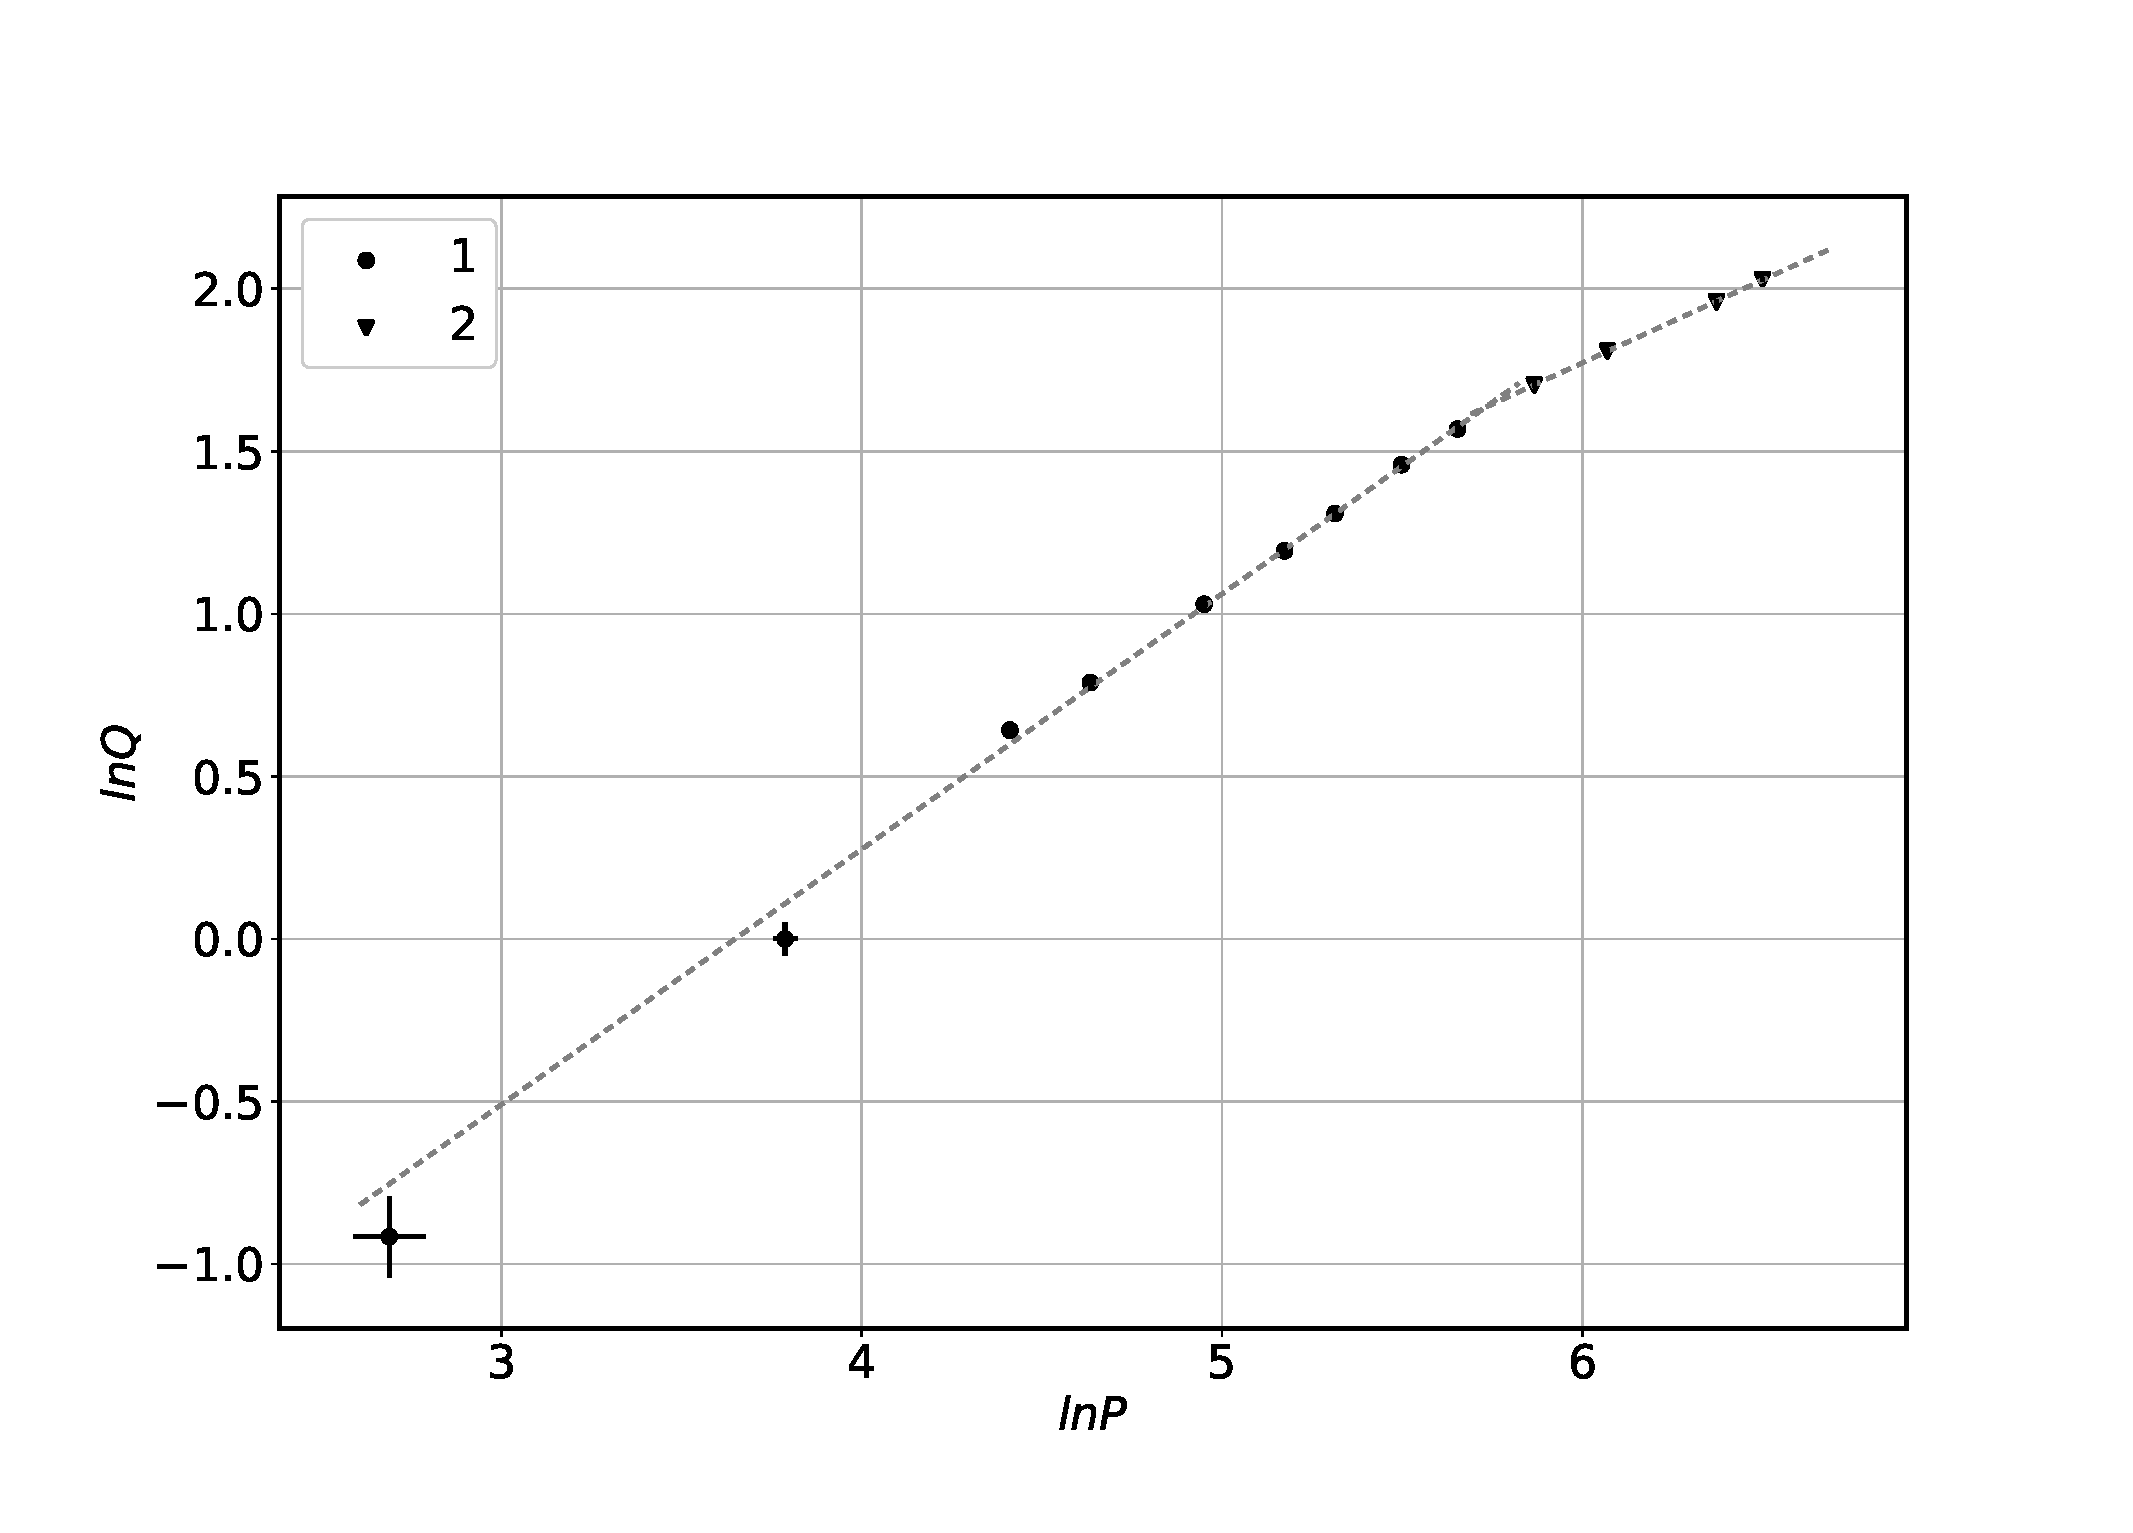
\includegraphics[width=0.8\textwidth]{lnPlnQd2.eps}
    \caption{Зависимость потока воздуха через трубку $Q$ в зависимости от перепада давления на концах
        трубки $P$. Диаметр трубки $d_2 = 3$ мм. Длина трубки $l_2 = 30$ см. Цифрами на графике обозначены 
        участки газа, удовлетворяющие различным режимам течения газа: 
        1 - ламинарное течение газа,
        2 - турбулентный переходное течение газа, 
        3 - турбулентное установившиеся течение газа.}
    \label{fig:lnPlnQd2}
\end{figure}
Для трубки диаметром $5.3$ мм графики зависимости $Q(P)$ (Рис.\ref{fig:PQd3} и \ref{fig:lnPlnQd3}) выглядят аналогично трубке с диаметром $3$ мм, 
на них также отсутствует переходной неустойчивый турбулентный режим, а ламинарное течение переходит сразу в 
устойчивое турбулентное. Однако для такой широкой трубки модель ламинарного течения уже не выполняется 
настолько же хорошо, как для более тонких трубок, потому зависимость при ламинарном течении на графике 
не является идеально прямой.
\begin{figure}[H]
    \centering
    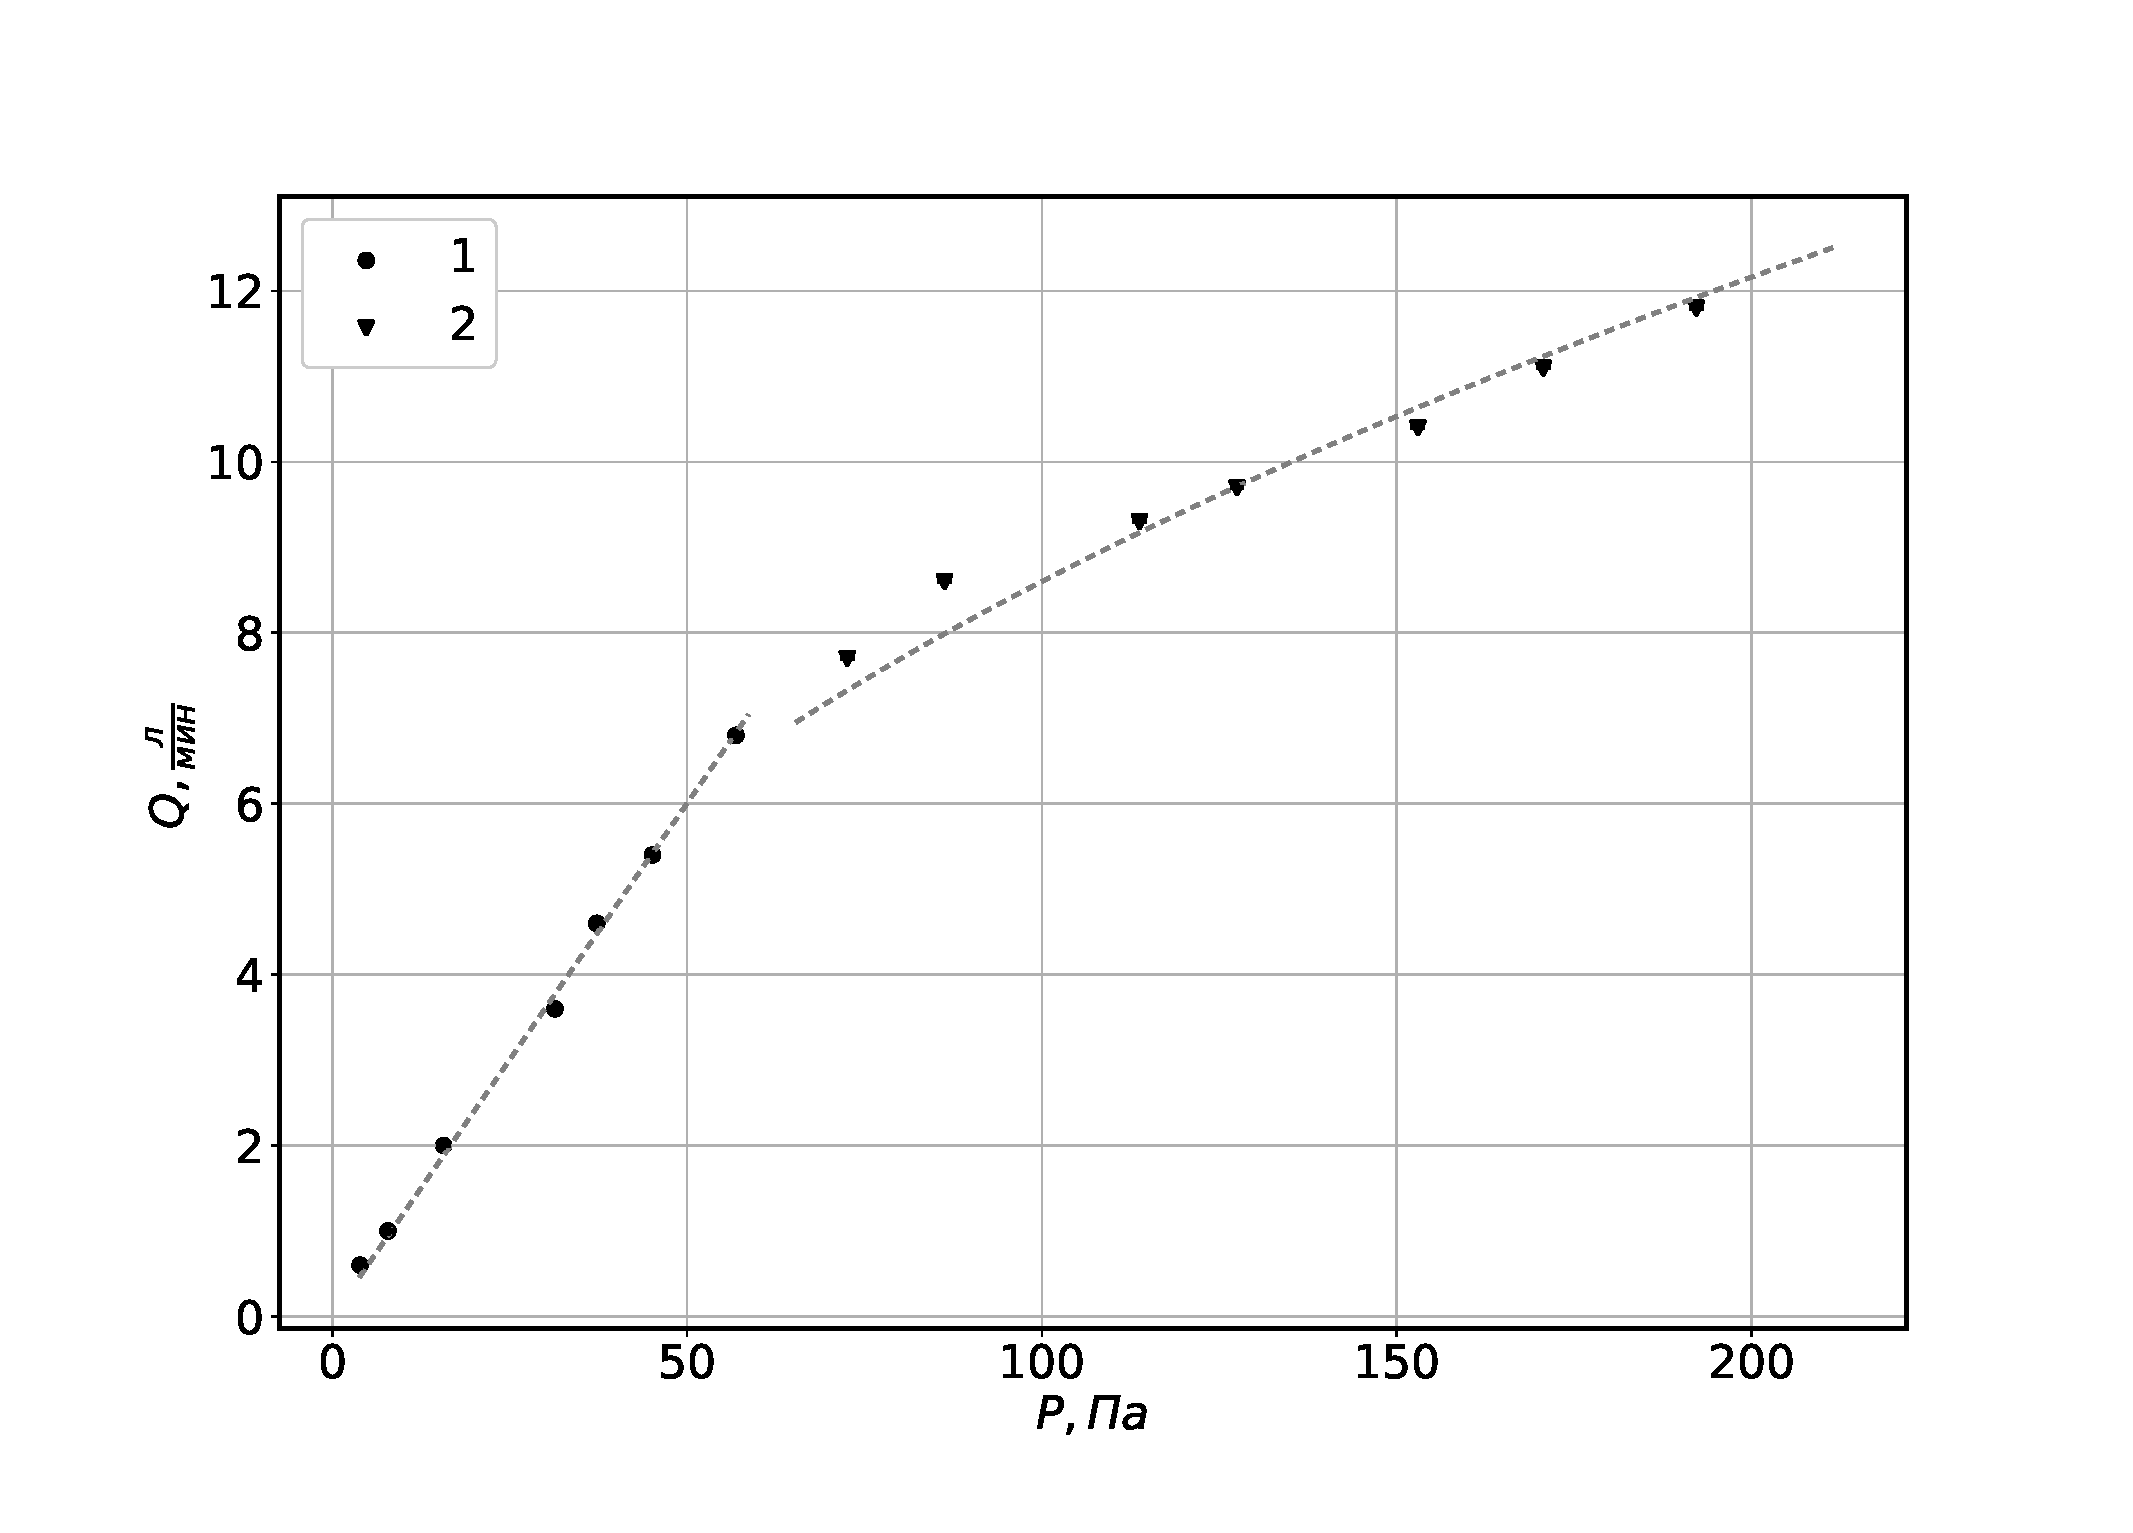
\includegraphics[width=0.8\textwidth]{PQd3.eps}
    \caption{Зависимость потока воздуха через трубку $Q$ в зависимости от перепада давления на концах
        трубки $P$. Диаметр трубки $d_3 = 5.3$ мм. Длина трубки $l_3 = 50$ см. Цифрами на графике обозначены 
        участки газа, удовлетворяющие различным режимам течения газа: 
        1 - ламинарное течение газа,
        2 - турбулентный переходное течение газа, 
        3 - турбулентное установившиеся течение газа.}
    \label{fig:PQd3}
\end{figure}
\begin{figure}[H]
    \centering
    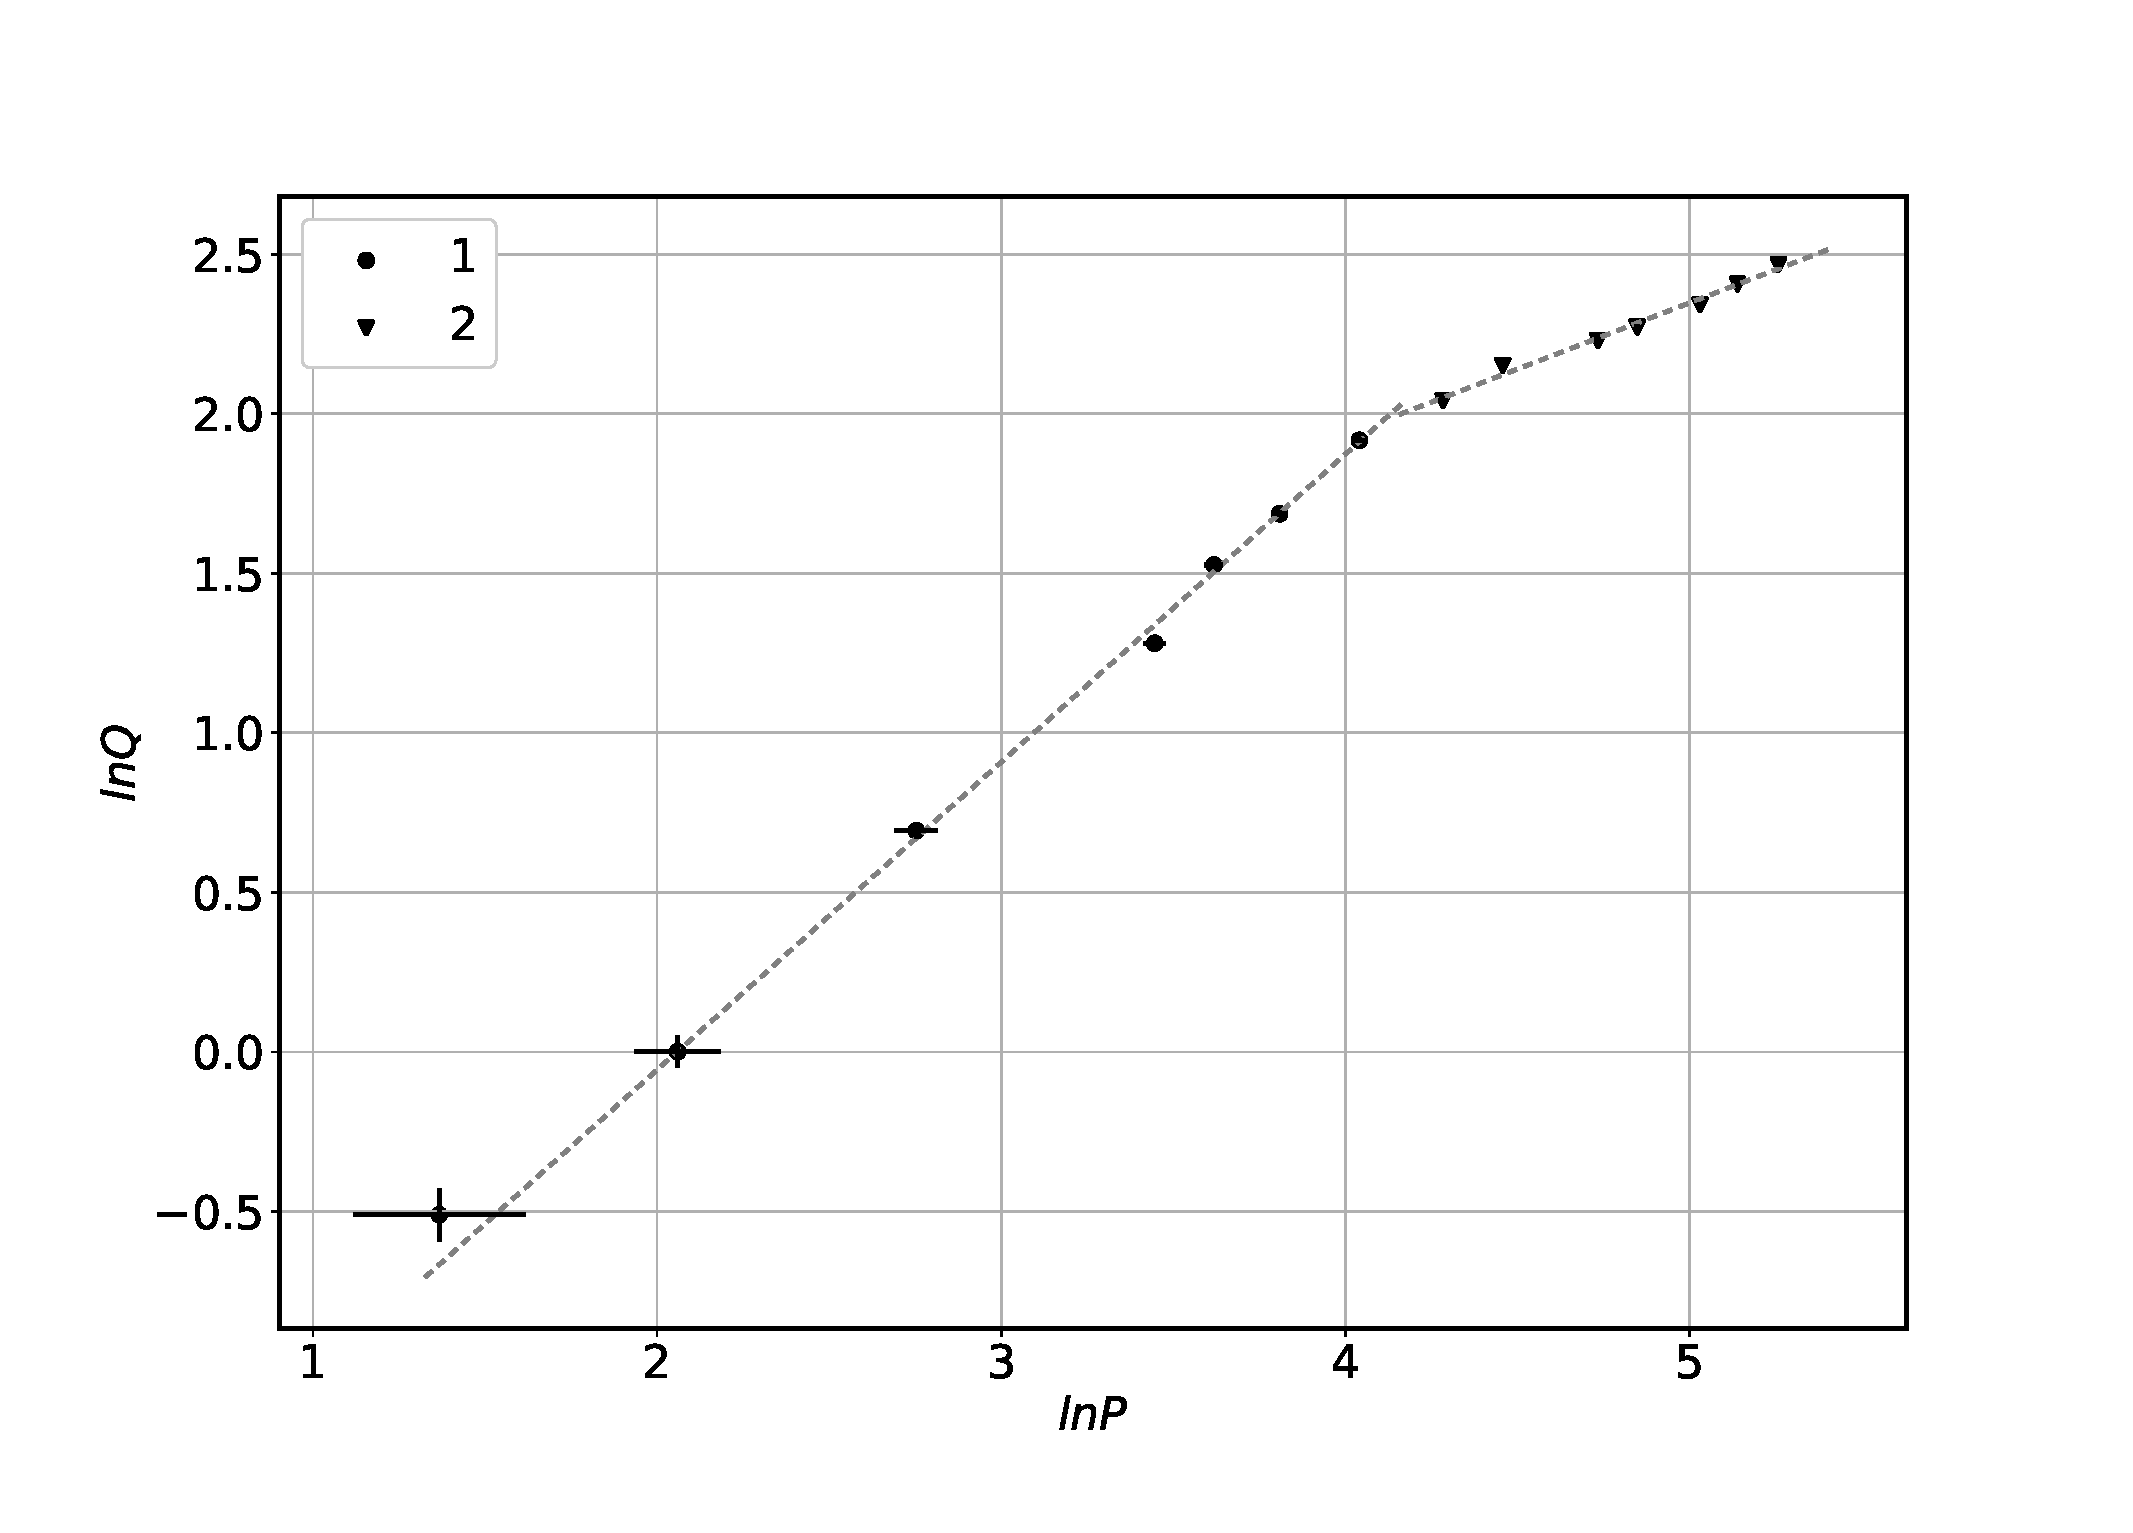
\includegraphics[width=0.8\textwidth]{lnPlnQd3.eps}
    \caption{Зависимость потока воздуха через трубку $Q$ в зависимости от перепада давления на концах
        трубки $P$. Диаметр трубки $d_3 = 5.3$ мм. Длина трубки $l_3 = 50$ см. Цифрами на графике обозначены 
        участки газа, удовлетворяющие различным режимам течения газа: 
        1 - ламинарное течение газа,
        2 - турбулентный переходное течение газа, 
        3 - турбулентное установившиеся течение газа.}
    \label{fig:lnPlnQd3}
\end{figure}
По полученным коэффициентам наклона прямых, характеризующих ламинарное течение газа для трубок различных 
диаметров расчитаны коэффициенты вязкости воздуха (Таблица \ref{tab:nus}). 
\begin{table}[H]
    \centering
    \begin{tabular}{|l|l|l|l|}
        \hline
        $d$, мм                          & 3.95 & 3.00 & 5.30                             \\
        \hline
        $\eta, \text{Па} \cdot \text{с}$ & $    &nu1& $    & $ &nu2& $ & $ &nu3& $ \\
        \hline
    \end{tabular}
    
    \caption{Результаты измерений сопростивления \(R\) от выделяемого тепла \(Q\) при температуре \(T = 23\)\textcelsius.
        Прямыми измерениями являются напряжение \(U\) и ток \(I\), \(\sigma Q\) и \(\sigma R\) - погрешности косвенных измерений.}
    \label{tab:nus}
\end{table}
Полученные значения слабо отличаются между собой, потому можно считать, что представленная модель корректно описывает 
ламинарное течение газа. 
\subsection*{Измерение распределения давления в трубке при ламинарном течении газа}
Для трёх трубок измерены перепады давления на различных их участках (Таблица \ref{tab:2}). 
расход при котором проводилось измерение подбирался так, чтобы течение в трубках оставалось ламинарным. 
По полученным данным построены графики зависимости давления $P$  в трубке от координаты измерения $x$ (Рис. \ref{fig:xP1}, \ref{fig:xP2}, \ref{fig:xP3}). 
\begin{figure}[H]
    \centering
    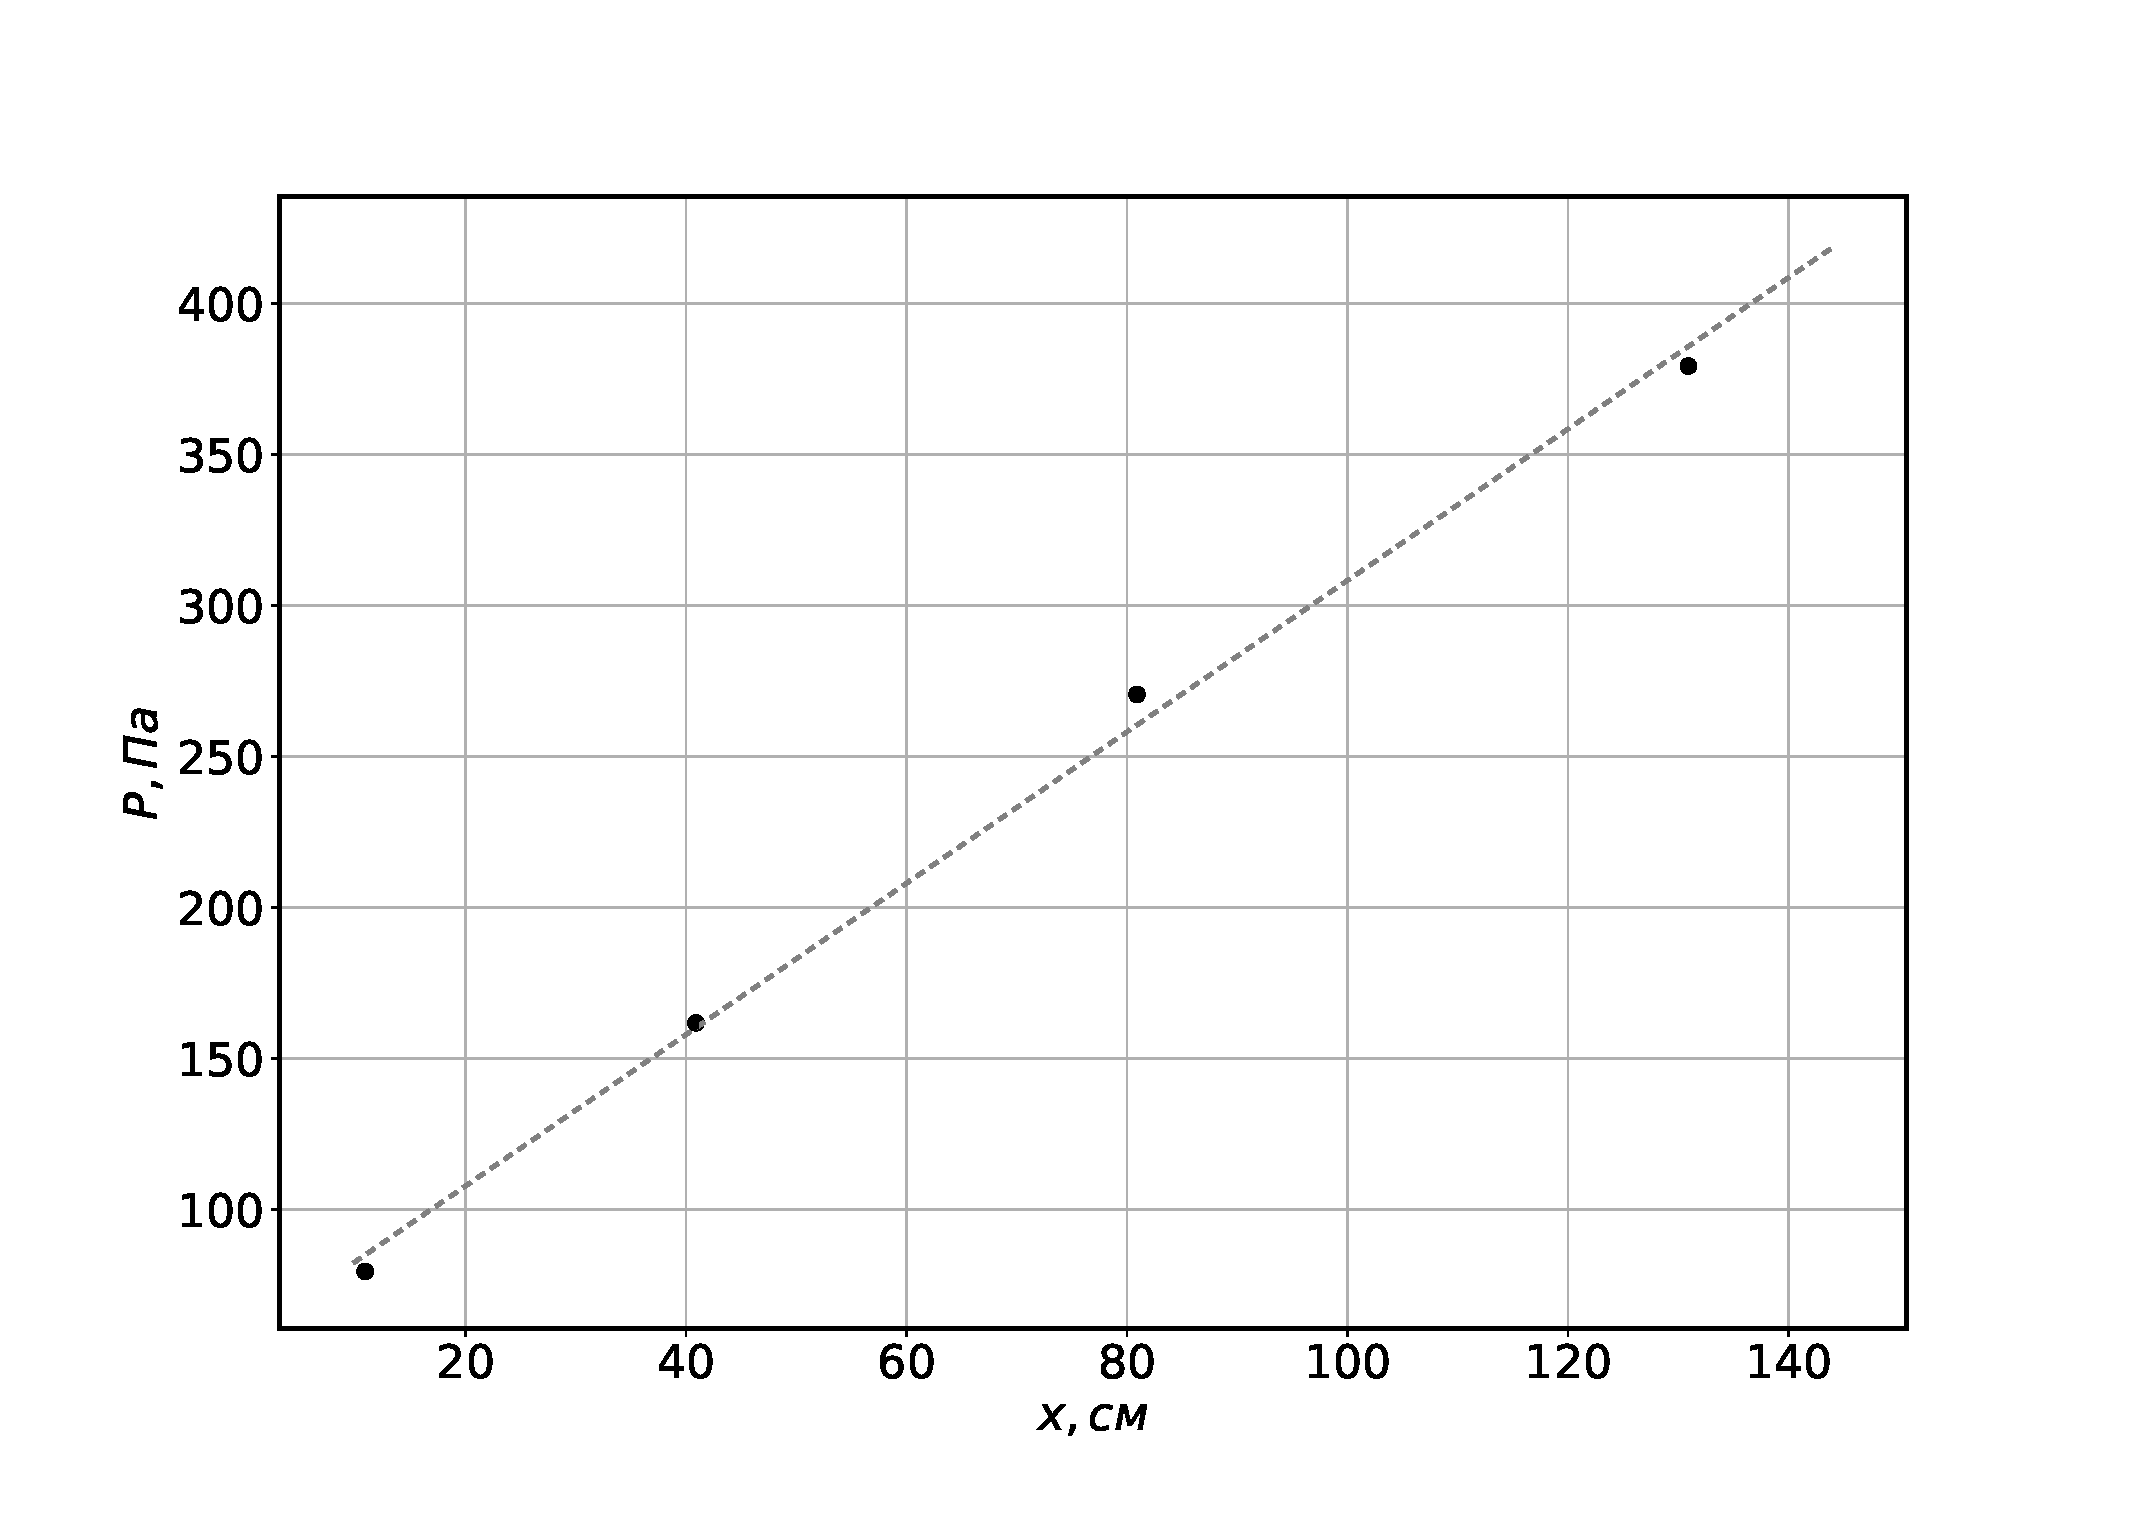
\includegraphics[width=0.7\textwidth]{xP1.eps}
    \caption{Зависимость давления $P$ в трубке от координаты измерения $x$, для трубки
        диаметром $d_1 = 3.95$ мм}
    \label{fig:xP1}
\end{figure}
\begin{figure}[H]
    \centering
    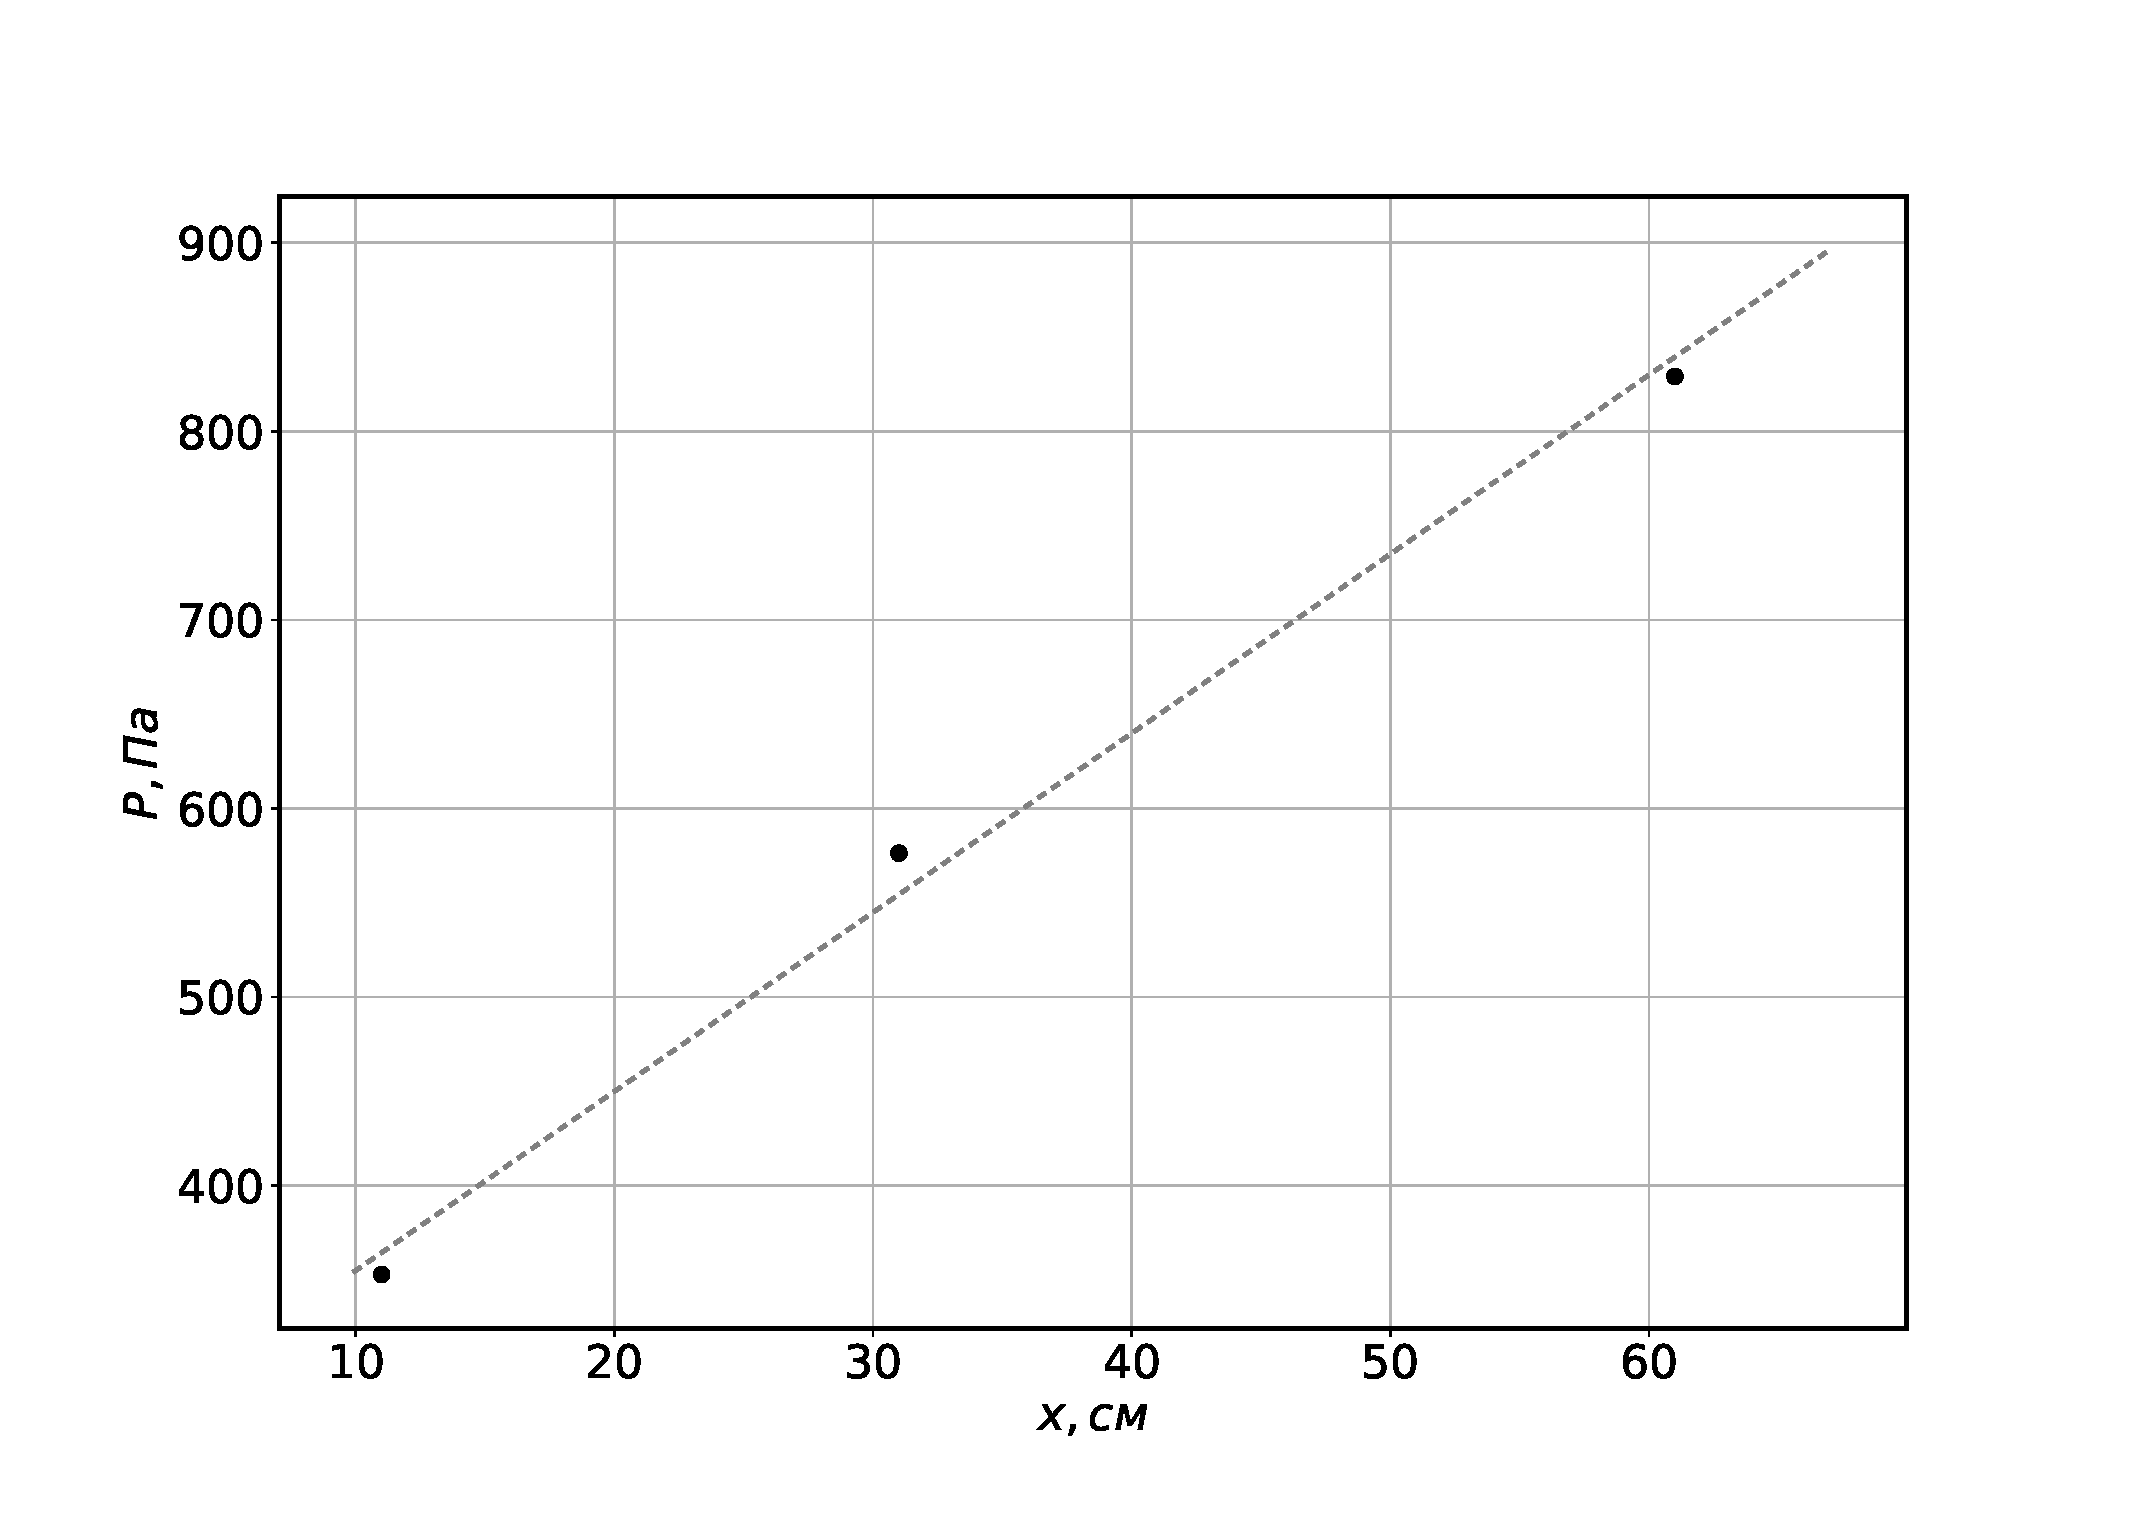
\includegraphics[width=0.7\textwidth]{xP2.eps}
    \caption{Зависимость давления $P$ в трубке от координаты измерения $x$, для трубки
        диаметром $d_2 = 3$ мм}
    \label{fig:xP2}
\end{figure}
\begin{figure}[H]
    \centering
    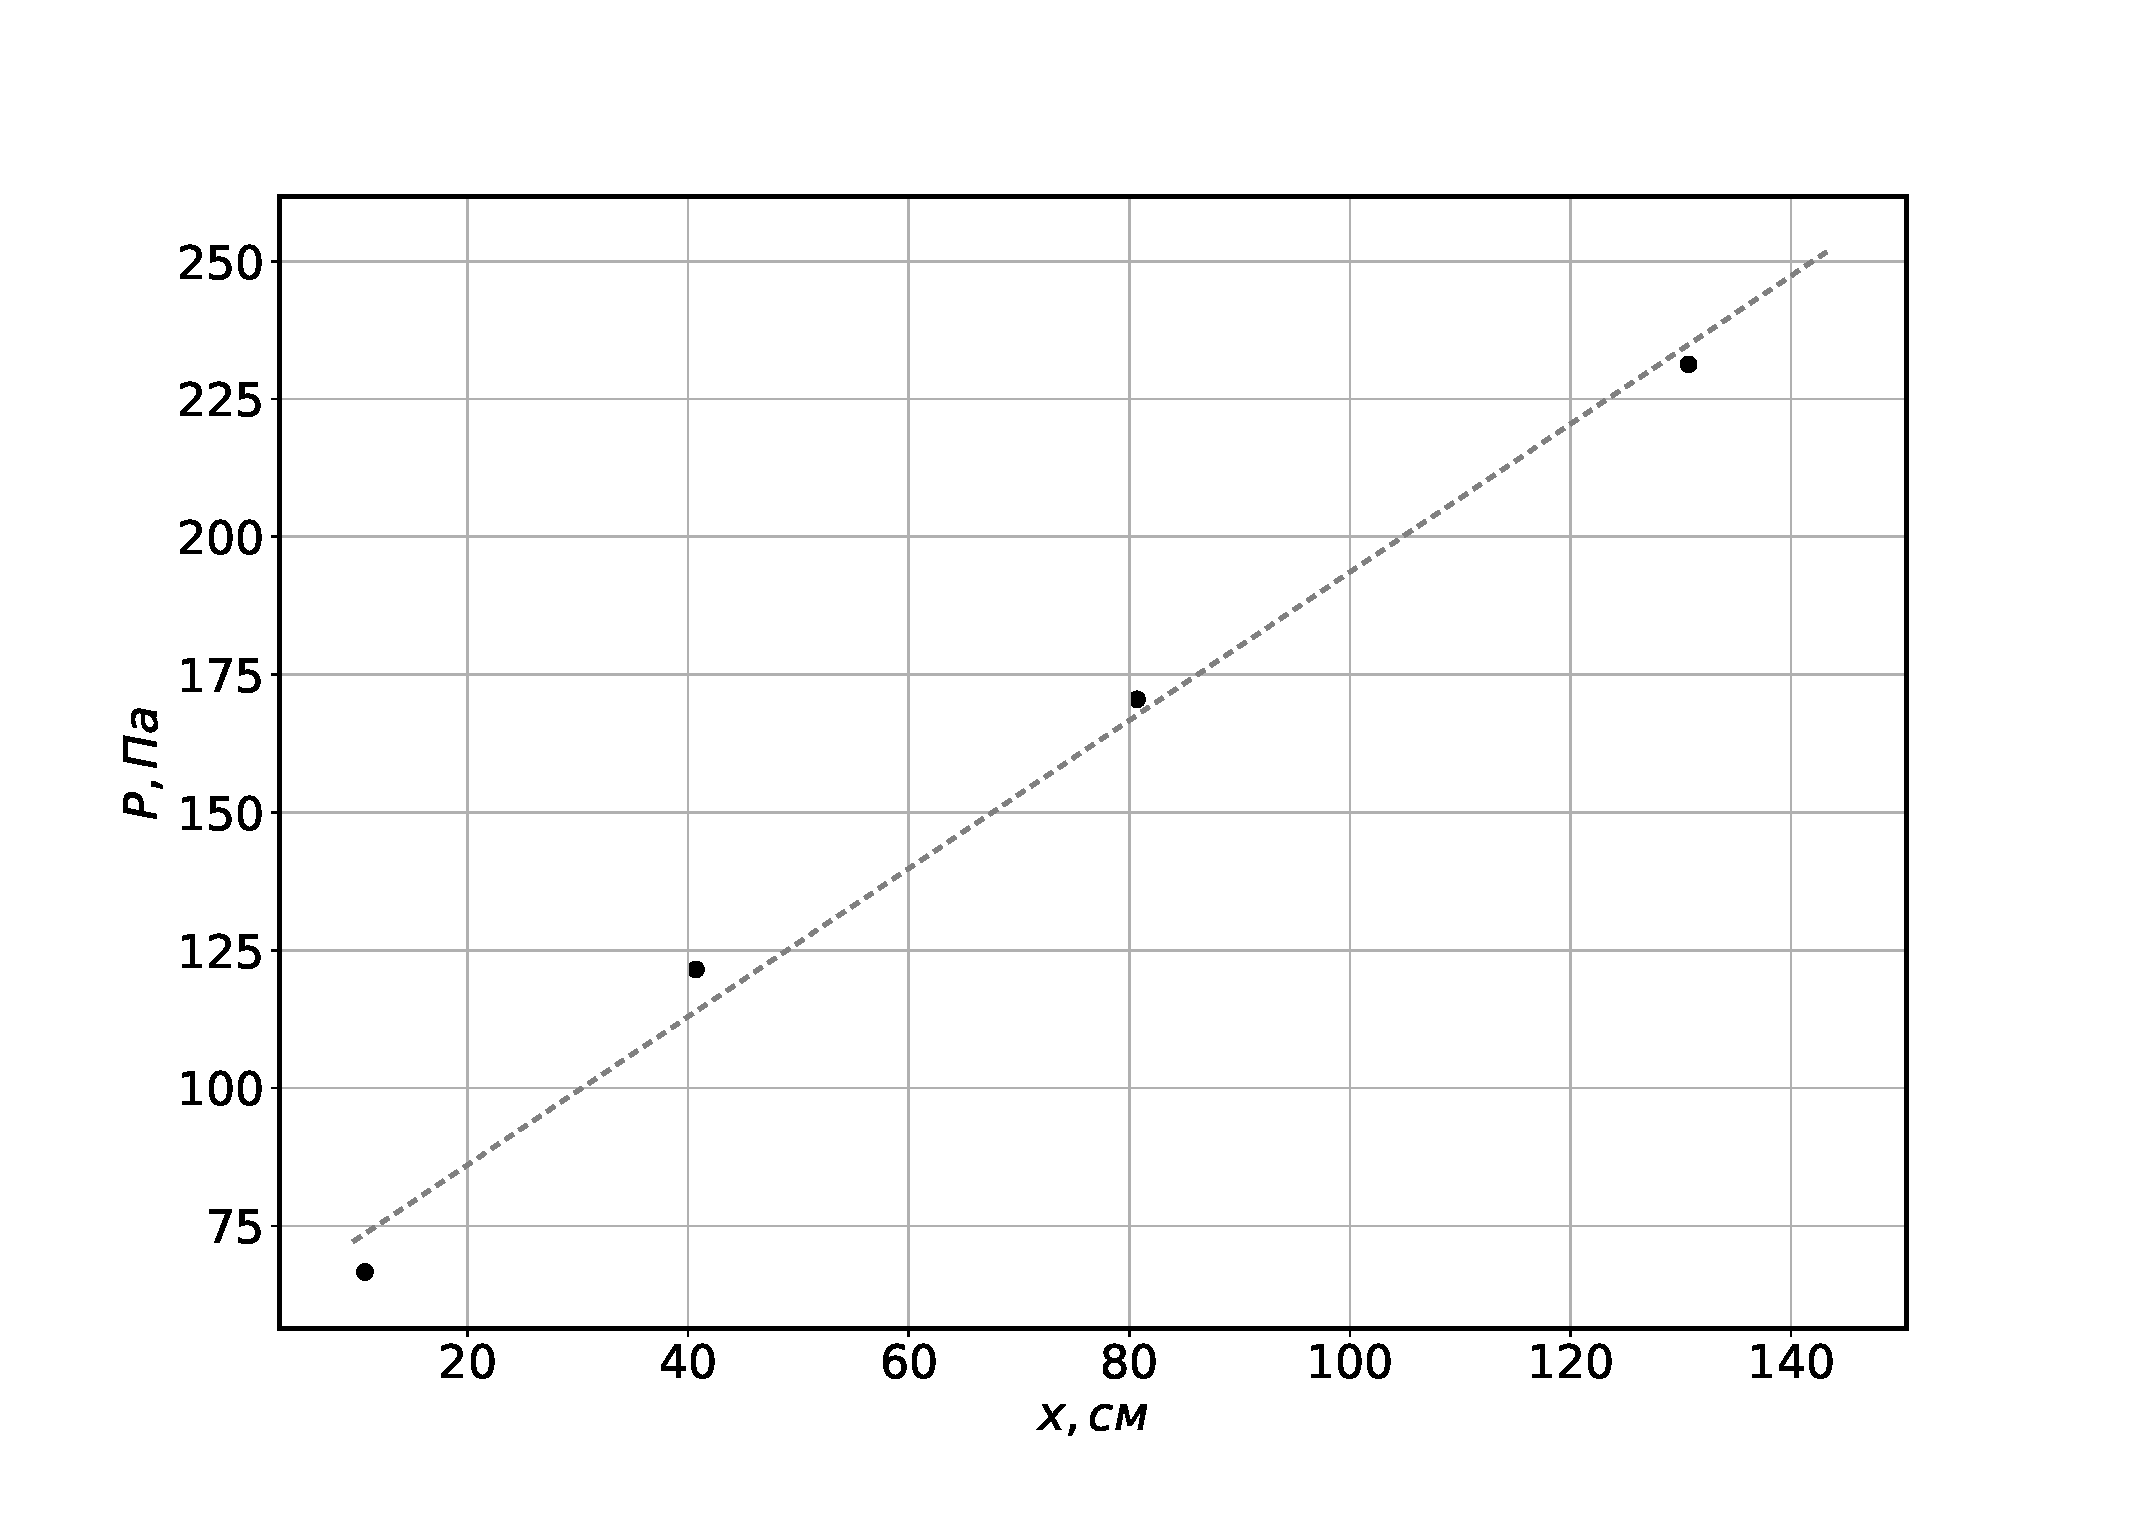
\includegraphics[width=0.7\textwidth]{xP3.eps}
    \caption{Зависимость давления $P$ в трубке от координаты измерения $x$, для трубки
        диаметром $d_3 = 5.3$ мм}
    \label{fig:xP3}
\end{figure}
Зависимость на всех графиках хорошо описывается линейной.
\section{Выводы}
Проведено измерение зависимости потока через тонкие трубки от перепада давления на их концах. 
Подтверждена теоретическая модель течения газа при низких и высоких перепадах давления. 
На основании модели ламинарного течения найден коэффициент вязкости воздуха. 
Установлен вид распределения давления в трубке при ламинарном течении газа.

\section{Использованная литература}
\begin{thebibliography}{9}
    \bibitem{LabBook}
    Лабораторный практикум по общей физике, Том 1, под редакцией А. Д. Гладуна
    \bibitem{Kirichenko}
    Н.А. Кириченко «Термодинамика, статистическая и молекулярная физика», п. 5.5
\end{thebibliography}

\section{Приложения}
\subsection{Параметры установки и погрешности приборов} \label{app_1}
При работе использовались три трубки различных диаметров: $d_1 = &d1&$ м, $d_2 = &d2&$ м, $d_2 = &d3&$ м. 
При проведении измерений в помещении было давление $P_0 = 996.4$ hPa, влажность $\rho_0 = 39.5 \%$ и 
температура $T_0 = 26.8$ \textcelsius.     
\subsection{Данные результатов измерений} \label{app_2}
\begin{table}[H]
    \centering
    \begin{tabular}{|r|r|r|r|r|r|}
        \hline
        \multicolumn{2}{|c|}{$d = 3.95$ мм, $l = 50$ см} & 
        \multicolumn{2}{|c|}{$d = 3.00$ мм, $l = 30$ см} & 
        \multicolumn{2}{|c|}{$d = 5.30$ мм, $l = 50$ см}                                                         \\
        \hline
        $Q$, л/мин                                       & $P$, Па & $Q$, л/мин & $P$, Па & $Q$, л/мин & $P$, Па \\
        \hline
        0.5                                              & 14      & 0.4        & 15      & 0.6        & 4       \\ 
        1.0                                              & 25      & 1.0        & 44      & 1.0        & 8       \\ 
        1.3                                              & 35      & 1.9        & 82      & 2.0        & 16      \\ 
        2.3                                              & 61      & 2.2        & 103     & 3.6        & 31      \\ 
        2.8                                              & 76      & 2.8        & 141     & 4.6        & 37      \\ 
        4.2                                              & 116     & 3.3        & 177     & 5.4        & 45      \\ 
        5.0                                              & 141     & 3.7        & 203     & 6.8        & 57      \\ 
        5.9                                              & 175     & 4.3        & 244     & 7.7        & 72      \\ 
        6.7                                              & 257     & 4.8        & 285     & 8.6        & 86      \\ 
        7.5                                              & 365     & 5.5        & 353     & 9.3        & 114     \\ 
        7.9                                              & 400     & 6.1        & 432     & 9.7        & 127     \\ 
        8.4                                              & 445     & 7.1        & 585     & 10.4       & 153     \\ 
        8.9                                              & 502     & 7.6        & 665     & 11.1       & 171     \\ 
        9.4                                              & 563     & -          & -       & 11.8       & 192     \\ 
        \hline
    \end{tabular}
    
    \caption{Результаты измерений объёмного расхода воздуха $Q$ в зависимости от перепада давления на
        концах трубки $P$. Результаты измерены на трёх трубках с диаметром $d$ и длиной $l$.}
    \label{tab:1}
\end{table}
\begin{table}[H]
    \centering
    \begin{tabular}{|r|r|r|r|r|r|r|r|r|}
        \hline
        \multicolumn{3}{|c|}{$d = 3.95$ мм, $Q = 4.3$ л/мин} & 
        \multicolumn{3}{|c|}{$d = 3.00$ мм, $Q = 4.3$ л/мин} & 
        \multicolumn{3}{|c|}{$d = 5.30$ мм, $Q = 7.1$ л/мин}                                                                                           \\
        \hline
        $x_1$, см                           & $x_2$, см & $P$, Па & $x_1$, см & $x_2$, см & $P$, Па & $x_1$, см & $x_2$, см & $P$, Па \\ 
        \hline
        40.9                                & 130.9     & 227     & 31.0      & 61.0      & 238     & 80.7      & 130.7     & 57      \\ 
        10.9                                & 130.9     & 315     & 11.0      & 61.0      & 470     & 40.7      & 130.7     & 110     \\ 
        0.0                                 & 130.9     & 379     & 11.0      & 31.0      & 229     & 10.7      & 130.7     & 163     \\ 
        0.0                                 & 80.9      & 270     & 0.0       & 61.0      & 829     & 0.0       & 130.7     & 231     \\ 
        0.0                                 & 40.9      & 162     & 0.0       & 31.0      & 576     & 40.7      & 80.7      & 47      \\ 
        0.0                                 & 10.9      & 79      & 0.0       & 11.0      & 353     & 10.7      & 80.7      & 102     \\ 
        40.9                                & 80.9      & 109     & -         & -         & -       & 0.0       & 80.7      & 171     \\ 
        10.9                                & 80.9      & 194     & -         & -         & -       & 10.7      & 40.7      & 53      \\ 
        10.9                                & 40.9      & 82      & -         & -         & -       & 0.0       & 40.7      & 122     \\ 
        -                                   & -         & -       & -         & -         & -       & 0.0       & 10.7      & 67      \\ 
        \hline
    \end{tabular}
    
    \caption{Результаты измерений перепада давления $P$ между точками с координатами $x_1$ и $x_2$.
        Данные получены для трёх различных труб с диаметрами $d$. Эксперимент для каждой трубы проводился при 
        объёмном расходе $Q$, подобранным таким образом, чтобы течение газа оставалось ламинарным.}
    \label{tab:2}
\end{table}
\end{document}